% \documentclass{book}

\documentclass[12pt]{article}
\usepackage[pdfborder={0 0 0.5 [3 2]}]{hyperref}%
\usepackage[left=1in,right=1in,top=1in,bottom=1in]{geometry}%
% \usepackage[shortalphabetic]{amsrefs}%
\usepackage{amsmath}
\usepackage{enumerate}
\usepackage{enumitem}
\usepackage{amssymb}               
\usepackage{amsfonts}
\usepackage{amsthm}
\usepackage{bbm}
\usepackage[table,xcdraw]{xcolor}
\usepackage{tikz}
\usepackage{float}
\usepackage{booktabs}
\usepackage{svg}
\usepackage{mathtools}
\usepackage{cool}
\usepackage{url}
\usepackage{graphicx,epsfig}
\usepackage{makecell}
\usepackage{array}

\usepackage{biblatex}
\addbibresource{NumericsReport.bib}

\def\noi{\noindent}
\def\T{{\mathbb T}}
\def\R{{\mathbb R}}
\def\N{{\mathbb N}}
\def\C{{\mathbb C}}
\def\Z{{\mathbb Z}}
\def\P{{\mathbb P}}
\def\E{{\mathbb E}}
\def\Q{\mathbb{Q}}
\def\ind{{\mathbb I}}

\newtheorem{theorem}{Theorem}

\graphicspath{ {images/} }

\begin{document}

\begin{center}
{\LARGE Numerical Evaluation of the Stability of Double Pulse Solutions to the 5th order KdV Equation}\\
\vspace{5mm}
{\large 5 June, 2017}\\
\end{center}

\section{Introduction}

The Kawahara equation is a fifth-order KdV-type equation which is used to model dispersive phenomena such as capillary-gravity water waves, plasma waves, and chains of coupled nonlinear oscillators \cite{Bridges2002,Champneys1998}. It takes the general form:

\begin{equation} \label{kawahara}
u_t + \alpha u_{xxx} + \beta u_{xxxxx} = \frac{\partial}{\partial x} f(u, u_x, u_{xx})
\end{equation}

If we take $\alpha = 1$, $\beta = 1$, and $f(u, u_x, u_{xx}) = -u^2$, we obtain the 5th order KdV equation \cite{Pelinovsky2007}. 

\begin{equation} \label{KdV5}
u_t = u_{xxxxx} - u_{xxx} - 2 u u_x
\end{equation}

We are interested in traveling wave solutions $u(x, t) = u(x - ct)$, where $c$ is the wave speed. Substituting this ansatz into \eqref{KdV5}, traveling wave solutions obey the equation

\begin{equation} \label{KdV5travel}
u_t = u_{xxxxx} - u_{xxx} + c u_x - 2 u u_x
\end{equation}

which can be written in the form

\begin{equation} \label{KdV5travelderiv}
u_t = \partial_x ( u_{xxxx} - u_{xx} + c u - u^2 )
\end{equation}

This equation \eqref{KdV5travelderiv} is Hamiltonian, and can be written as $u_t = J E'(u)$, where $J = -\partial / \partial_x$ and $E'(u)$ is the variational derivative of the Hamiltonian energy

\begin{equation} \label{Hamiltonian}
E(u) = -\int_{-\infty}^{\infty} \left( \frac{1}{2}u_{xx}^2 + \frac{1}{2}u_x^2 + \frac{1}{2}cu^2 - \frac{1}{3}u^3 \right) dx
\end{equation}

If we assume that the solution $u(x, t)$ and its first four derivatives decay to 0 at $\pm \infty$, we can show that the square of the $L^2$ norm of the solution is conserved, i.e. $\frac{\partial}{\partial t}N(u) = 0$, where

\begin{equation} \label{L2norm}
N(u) = \frac{1}{2} \int_{-\infty}^\infty u(x)^2 dx
\end{equation}

To verify this, 

\begin{align*}
\frac{\partial}{\partial t} N(u) &= \int_{-\infty}^\infty u u_t dx \\
&= \int_{-\infty}^\infty \left( u u_{xxxxx} - u u_{xxx} + c u u_x - 2u^2 u_x\right) \\
&= \int_{-\infty}^\infty \left( u_{xx} u_{xxx} + u_x u_{xx} + c u u_x - 2u^2 u_x\right) dx \\
&= \int_{-\infty}^\infty \frac{\partial}{\partial x} \left( \frac{1}{2} u_{xx}^2 + \frac{1}{2} u_x^2+ \frac{1}{2} c u^2 - \frac{2}{3} u^3 \right)\\
&= 0 
\end{align*}
where in the second line we substituted the PDE \eqref{KdV5}, in the third line we integrated by parts (boundary terms are zero since we assume the solution $u(x, t)$ and its first four derivatives decay to 0 at $\pm \infty$), and in the penultimate line, the integral of the exact differential is zero for the same reason.\\

For an equilibrium solution to \eqref{KdV5travel}, we have $u_t = 0$. We can then integrate \eqref{KdV5travelderiv} once, using boundary conditions of 0 on $u$ and its first four derivatives as $x \rightarrow \pm \infty$ to get the 4th order nonlinear ODE

\begin{equation} \label{intKdV}
u_{xxxx} - u_{xx} + c u - u^2 = 0
\end{equation}

Suppose $u^*(x)$ is a solution to \eqref{intKdV}, i.e. it is an equilibrium solution to \eqref{KdV5travel}. Then we can linearize \eqref{intKdV} about the solution $u^*(x)$ to obtain the eigenvalue problem $Hv = \lambda v$, where $H$ is a linear operator on $L^2(\R)$ (I THINK WE ARE OK HERE WITH $L^2$ SINCE WE HAVE DERIVATIVES IN THE WEAK SENSE, BUT THIS COULD ALSO BE $H^4$) given by

\begin{equation}\label{linear4th}
H = E''(u) = \partial_x^4 - \partial_x^2 + c - 2 u^*
\end{equation}
i.e. the operator $H$ is the Hessian of the energy $E$.\\

Similarly, we can linearize the 5th order PDE \eqref{KdV5travel} about the solution $u^*(x)$ to obtain the eigenvalue problem $Lv = \lambda v$, where $L$ is a linear operator on $L^2(\R)$ given by

\begin{equation}\label{linear5th}
L = \partial_x^5 - \partial_x^3 + (c - 2 u^*) \partial_x - 2 u^*_x
\end{equation}

Most of the references below I got from Chugunova \cite{Pelinovsky2007}. For an actual paper, I will check these references (and others) more carefully.\\

The existence of localized solutions which are homoclinic orbits connecting the solution $u(x) = 0$ to itself has been shown \cite{Champneys1998}. For wave speed $c > 0$, the equation \eqref{intKdV} has a one-pulse solution (up to translation). Linearization of \eqref{intKdV} about the zero solution $u(x) = 0$ leads to the the eigenvalue equation
\begin{equation} \label{charpoly1}
\nu^4 - \nu^2 + c = 0
\end{equation}

For $0 < c < 1/4$, the four roots of \eqref{charpoly1} are all real, and the one-pulse solution is the only localized solution to \eqref{intKdV} \cite{Groves1997}. For the specific value $c = 36/169 < 1/4$, the analytical form of the one-pulse solution is known \cite{Pelinovsky2007}.

\begin{equation} \label{exact}
u(x) = \frac{105}{338}\textrm{sech}^4\left(\frac{x}{2\sqrt{13}} \right)
\end{equation}

For $c > 1/4$, the roots of \eqref{charpoly1} are complex and are of the form
\begin{equation} \label{alphabeta}
\nu = \pm \alpha \pm i \beta
\end{equation}
where $\beta \neq 0$. In this case, the equation \eqref{intKdV} has infinitely may multipulse solutions in addition to the single pulse solution. All localized solutions have  exponentially-decaying, oscillatory tails. Multipulse solutions resemble (to leading order) multiple copies of the single pulse solution.\\

In this paper, we will construct two-pulse solutions to \eqref{intKdV}, look at the spectrum of the linearization of \eqref{intKdV} and \eqref{KdV5travel} about these solutions, and perform timestepping starting at perturbations of these double pulse solutions.

\section{Numerics}

We start by finding solutions to the 4th order ODE \eqref{intKdV}. We use two different spectral methods for our spatial discretization and numerical differentiation. In both cases, the domain of discretization is $[-L, L] = [-25, 25]$.

\begin{enumerate}
	\item Fourier collocation method with periodic boundary conditions. We use $N = 256$ equally spaced grid points. (Mesh size is $h = 50 / 257$, since the endpoint at $x = 25$ is identified with the point $x = -25$). Differentiation matrices were computed using \texttt{fourdif} from \cite{Weideman2000}.
	\item Chebyshev collocation method. We use $N = 257$ grid points. Since we are solving a 4th order problem, we use homogeneous Dirichlet and Neumann boundary conditions at both ends, i.e. $u(\pm L) = u_x(\pm L) = 0$. To enforce these, we follow the method in \cite{Trefethen2000} and write our interpolation polynomial as
	\begin{equation}
		p(x) = \left[ 1 - \left(\frac{x}{L}\right)^2\right]q(x)
	\end{equation}
	and look for the unique polynomial $q(x)$ of degree $\leq N-2$ such that $q(\pm L) = 0$ and $q(x_j) = u(x_j) / (1 - (x_j / L)^2)$ for $j = 1, \dots, N-1$, where the $x_j$ are the Chebyshev Gauss-Lobatto collocation points. This polynomial satisfies both homogeneous Dirichlet and Neumann boundary conditions at both endpoints.
\end{enumerate}

\subsection{Parameter Continuation}

We start with the known solution \eqref{exact}, which solves \eqref{intKdV} as well as \eqref{KdV5travel} for $c = 36/169$. We choose one of the two spectral methods above (Fourier or Chebyshev) for spatial discretization. Using this solution on $[-L, L] = [-25, 25]$ as our initial guess, we use Matlab's \texttt{fsolve} to solve \eqref{intKdV} numerically using the appropriate discretization scheme and boundary conditions. Since both the original 5th order PDE \eqref{KdV5travel} and the 4th order stationary ODE \eqref{intKdV} are translation-invariant, these equations do not have unique solutions. In the 4th order case, that means that if $u(x)$ is a solution of \eqref{intKdV}, so is $u(x - a)$ for any $a \in \R$. Since we would like our numerical scheme to have a unique solution, and since the known solution \eqref{exact} is an even function, we modify our scheme to solve the following system of equations:
\begin{align}\label{intKdVsymm}
u_{xxxx} - u_{xx} + c u - u^2 &= 0 \\
\int_{-\infty}^\infty \left[ u(x) - u(-x) \right]^2 dx &= 0
\end{align}
where the second equation enforces even symmetry. This ensures that we have a unique solution. For our discretization, the integral in \eqref{intKdVsymm} is replaced by a sum, i.e. the discrete $L^2$ norm.\\

Starting with the solution for $c = 36/169$ which satisfies \eqref{intKdVsymm} and the appropriate boundary conditions for the spectral method we are using, we use the the method of parameter continuation (reference to NUMERICAL CONTINUATION, AND COMPUTATION OF NORMAL FORMS, Beyn et al, not sure where this is published) for the system \eqref{intKdVsymm}, where the wave speed $c$ is the parameter. Using this method, we increase $c$ by small increments until we reach $c = 10$. Here are plots of the single pulses constructed using this technique, together with a plot showing the linear relationship between the height of the single pulse and the wave speed.

\begin{figure}[H]
	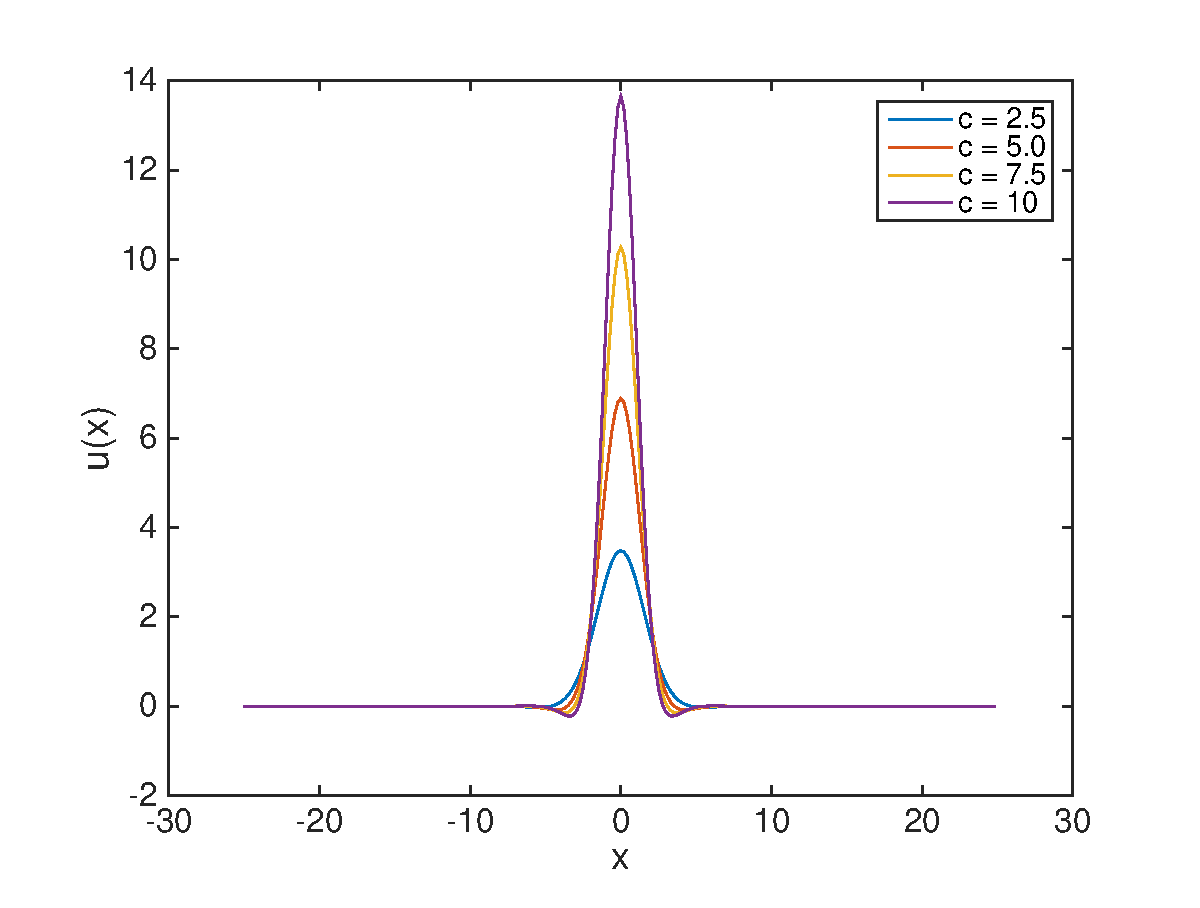
\includegraphics[width=8.5cm]{continuation.eps}
	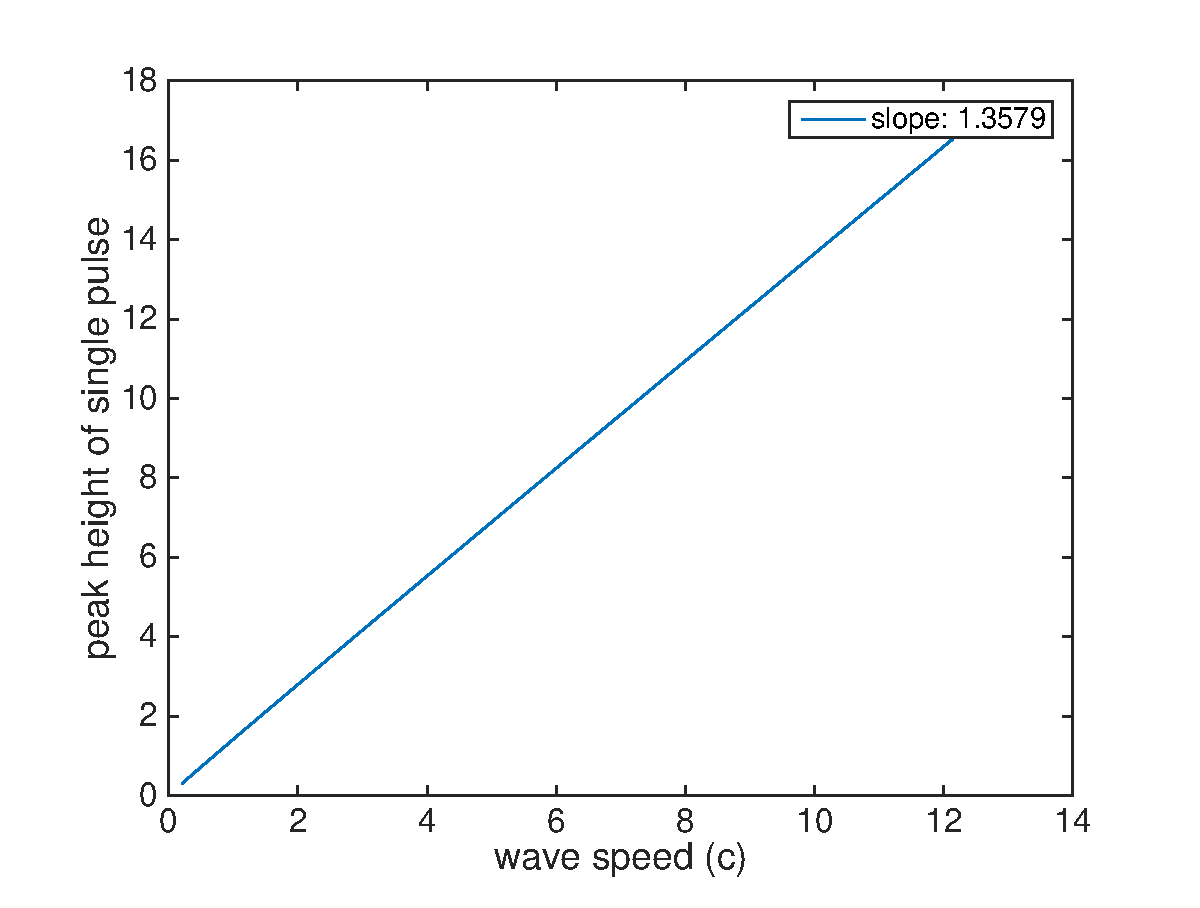
\includegraphics[width=8.5cm]{heightvsspeed.eps}
	\caption{Results of parameter continuation of single pulse solutions to 4th order ODE \eqref{intKdV} for four different wave speeds (left) and linear relationship between peak height and wave speed (right). Fourier spectral methods, $N = 256$.}
\end{figure}

For $c = 10$, we look at the exponentially decaying tail of the single pulse. For this value of $c$, the roots of the characteristic polynomial \eqref{charpoly1} are $\pm \alpha + \beta i = \pm1.3532 \pm 1.1537i$. We expect $\alpha$ to represent the exponential decay rate of the tails, and $\beta$ to be the frequency of oscillations. The plots below show that this is indeed the case.

\begin{figure}[H]
	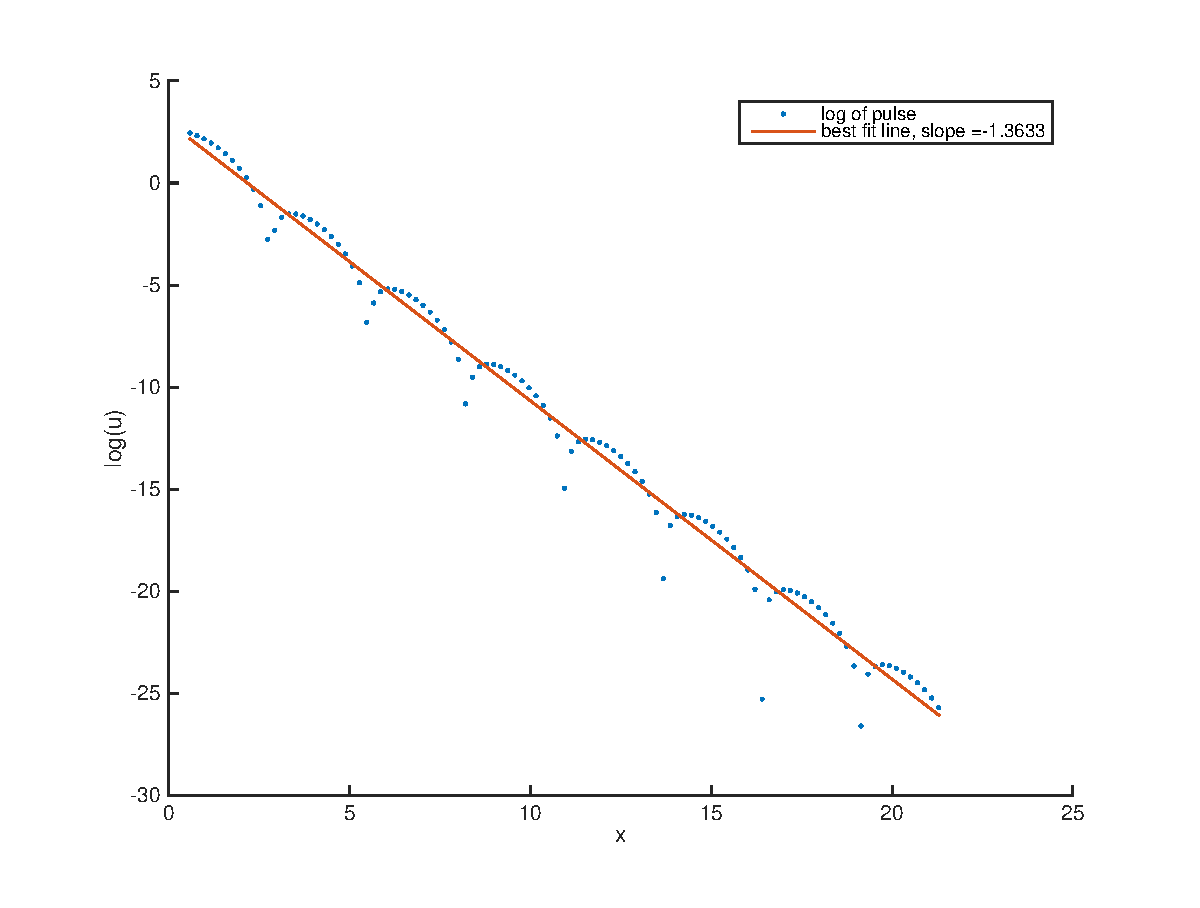
\includegraphics[width=8.5cm]{decaysinglepulse.eps}
	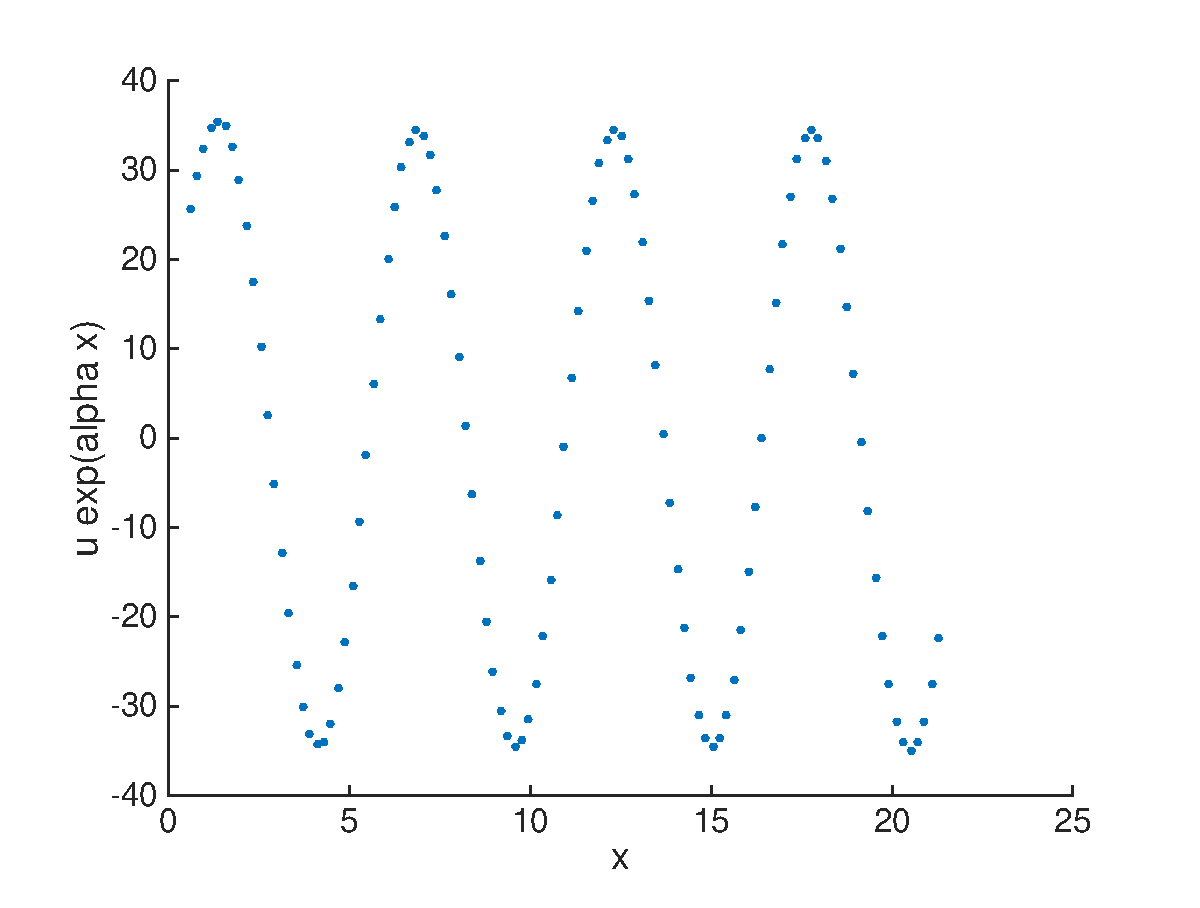
\includegraphics[width=8.5cm]{oscsinglepulse.eps}
	\caption{For single pulse $u(x)$, plot of $\log u(x)$ (left) and $e^{\alpha x} u(x)$ (right). Slope of best fit line on left is -1.3633, which is approximately $\alpha$. Period on right is 5.4688, frequency is 1.1489, which is approximately $\beta$. Wave speed $c = 10$, Fourier spectral methods, $N = 256$.}
\end{figure}

\subsection{Double Pulse Construction}

To construct double pulses numerically, we paste together two copies of the single pulse and use that as the initial guess for Newton's method. We classify double pulses following the notation in Theorem 3.6 in \cite{Sandstede1997}. The equation studied in \cite{Sandstede1997} is
\begin{equation}\label{strut}
u_{xxxx} + Pu_{xx} + u - u^2 = 0
\end{equation}
which is used to model equilibrium states of a strut. If we take $P = -1$ in this equation, we obtain our equation \eqref{intKdV} for wave speed $c = 1$. Multipulse solutions occur for $P \in (-2, -2 + \eta)$ for some $\eta > 0$, and should in fact occur for $P \in (-2, 2)$, which inclues $P = -1$. Although this equation only corresponds to wave speed $c = 1$, this should generalize to other values of $c$. (I ASSUME THIS IS TRUE, BUT IN ANY CASE, WE ARE ONLY USING THIS FOR NOTATION). We now rewrite Theorem 3.6 for the specific case of double pulses. Since we are not interested in the eigenvalue problem here, we omit that portion of the theorem for simplicity.

\begin{theorem}
Let $q(x)$ be a transversely constructed localized solution of \eqref{strut}. Assume that the following hypotheses hold:
\begin{enumerate}
	\item The spectrum of the linearization about the solution $u(x) = 0$ contains simple eigenvalues $\pm \alpha \pm i \beta$ for some $\alpha, \beta > 0$.
	\item I DON'T THINK WE NEED THE CONSERVATIVE ASSUMPTION (3.3), SINCE THIS EQUATION IS HAMILTONIAN; THE  HAMILTONIAN IS GIVEN ON P.2083 OF \cite{Sandstede1997}.
	\item I DON'T THINK WE NEED THE MELNIKOV ASSUMPTION (3.5) SINCE WE ARE NOT CONCERNED WITH THE EIGENVALUE PROBLEM HERE.
\end{enumerate}
Then there exists an $N_0 \in \N$ such that for all $n \geq N_0$, there is a 2-pulse solution $q_n(x)$ of \eqref{strut}. The 2-pulse solution $q_n(x)$ resembles two copies of the single pulse $q(x)$, and the distance between the pulses is given by
\begin{equation}\label{pulsedistance}
L_n = L + \frac{\pi}{\beta}n + r(n)
\end{equation}
where $L$ is a constant, and $r(n) \rightarrow 0$ as $n \rightarrow \infty$. IN THE PAPER \cite{Sandstede1997}, THERE ARE TWO CHAINS OF PULSES SEPARATED BY $2 \pi / \beta$ (TO LEADING ORDER) WHOSE STARTING POINTS ARE SEPARATED BY $\pi / \beta$; ONE CHAIN HAS POSITIVE EIGENVALUES, THE OTHER NEGATIVE. I ELECTED TO COMBINE THEM FOR EASIER NOTATION. WE ALSO MIGHT NOT NEED THE $N_0$ SINCE WE CAN JUST FOLD THAT INTO THE CONSTANT.
\end{theorem}

We will therefore label our double pulses using the notation $2(n)$, where $n$ is the natural number appearing in the theorem above; $n = 1$ corresponds to the double pulse where the two peaks are the closest. This is consistent with the notation in \cite{Champneys1993}.\\

To construct pulse 2(2) numerically, we first glue two single pulses at the first minimum of the tail. For each subsequent double pulse, we go another $\pi / 2 \beta$ further down the tail (away from the pulse) and glue the pulses there. For double pulse 2(1), we go $\pi / 2 \beta$ up the tail (towards the pulse) and glue the pulses there. We then use that glued double pulse as an inital guess and use Matlab's \texttt{fsolve} to find a solution of \eqref{intKdVsymm}, i.e. \eqref{intKdV} with a symmetry condition. The next plot shows the initial guess from gluing together with the output of \texttt{fsolve} for double pulse 2(2).

\begin{figure}[H]
	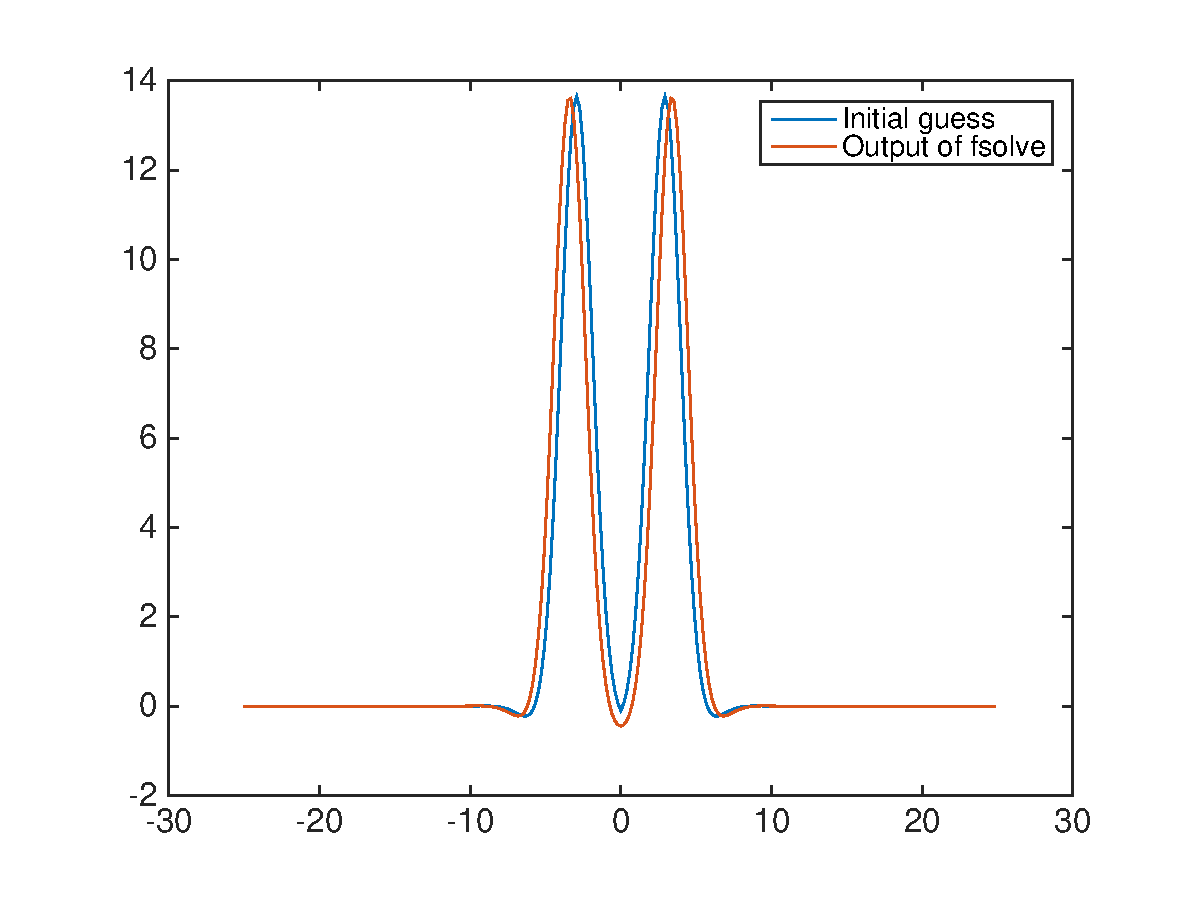
\includegraphics[width=8.5cm]{doublepulseconstruction}
	\caption{Constuction of double pulse 2(2). Initial guess and output of \texttt{fsolve} are shown. Fourier spectral methods, $N = 256$, wave speed $c = 10$.}
\end{figure}

Here are plots of the first five double pulses generated in this manner, both for Fourier and for Chebyshev spectral methods. Note that for double pulse 2(1), the two pulses overlap.

\begin{figure}[H]
	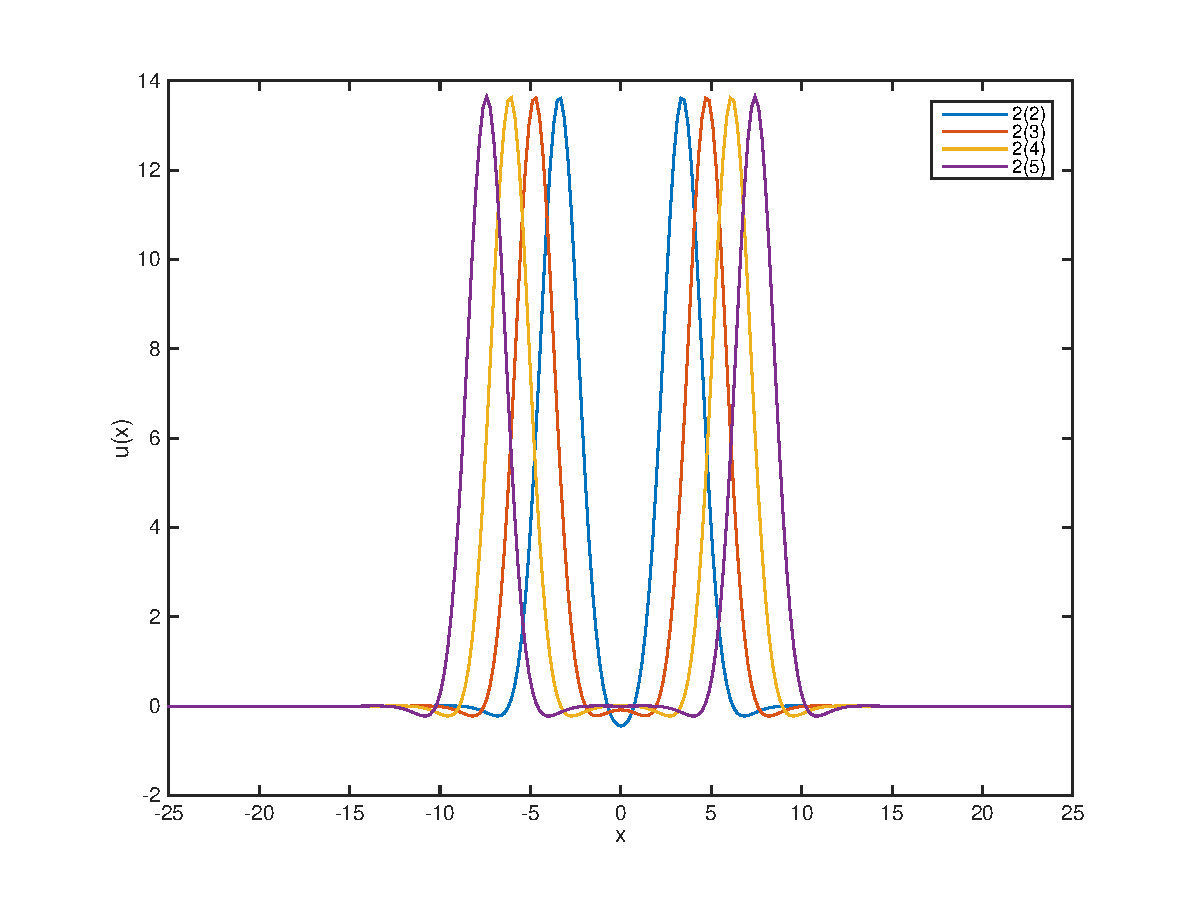
\includegraphics[width=8.5cm]{four10double.eps}
	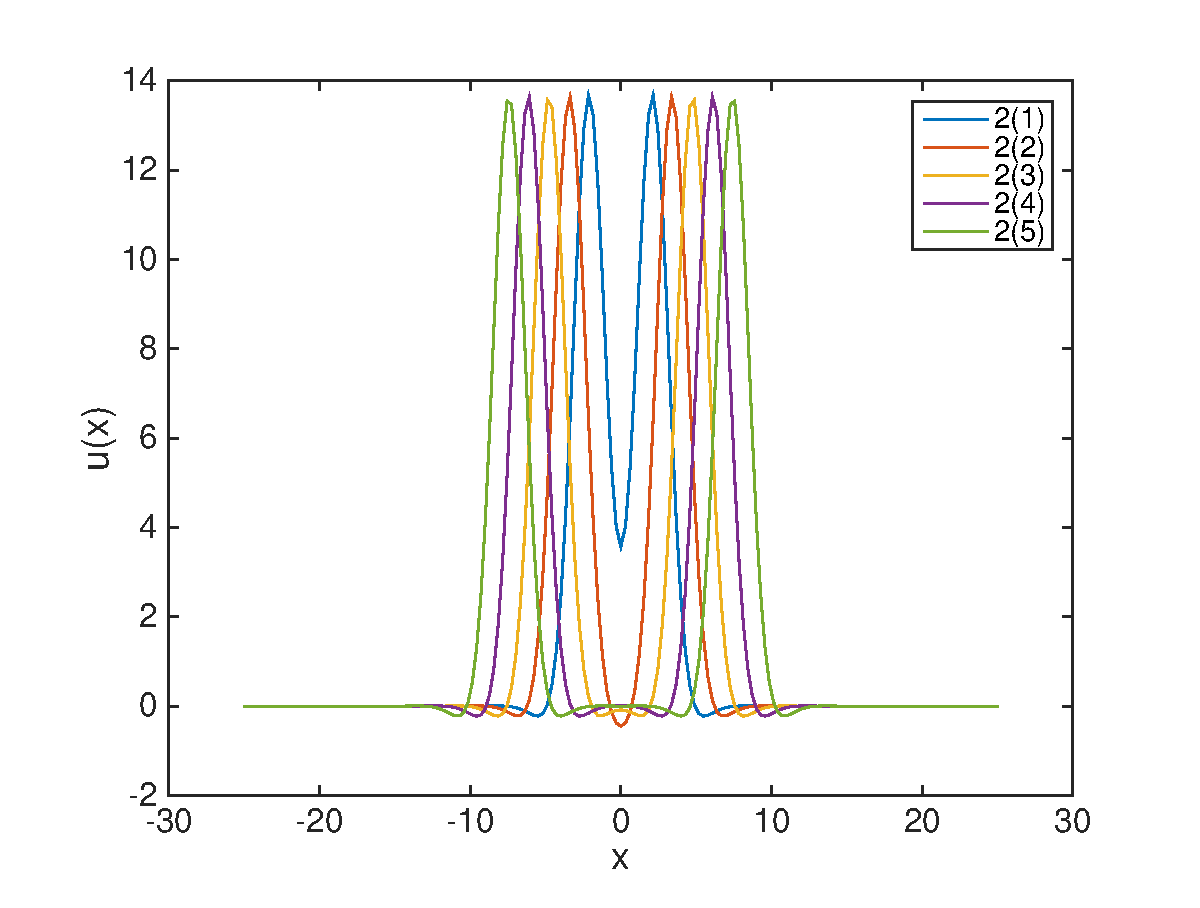
\includegraphics[width=8.5cm]{cheb10double}
	\caption{Primary pulse and double pulses 2(1), 2(2), 2(3), 2(4), and 2(5). Fourier spectral methods, $N = 256$, wave speed $c = 10$ (left). Chebyshev spectral methods, $N = 257$, wave speed $c = 10$ (right). }
\end{figure}

The following plot shows the difference between the solutions obtained from the two methods. Since the Chebyshev method uses a nonuniform grid while the Fourier method uses a uniform grid, we interpolated the Fourier data onto the Chebyshev grid using a cubic spline before subtracting. The difference between the two methods it as most of the order 1e-4, with the differerence slightly smaller for a larger domain size.

\begin{figure}[H]
	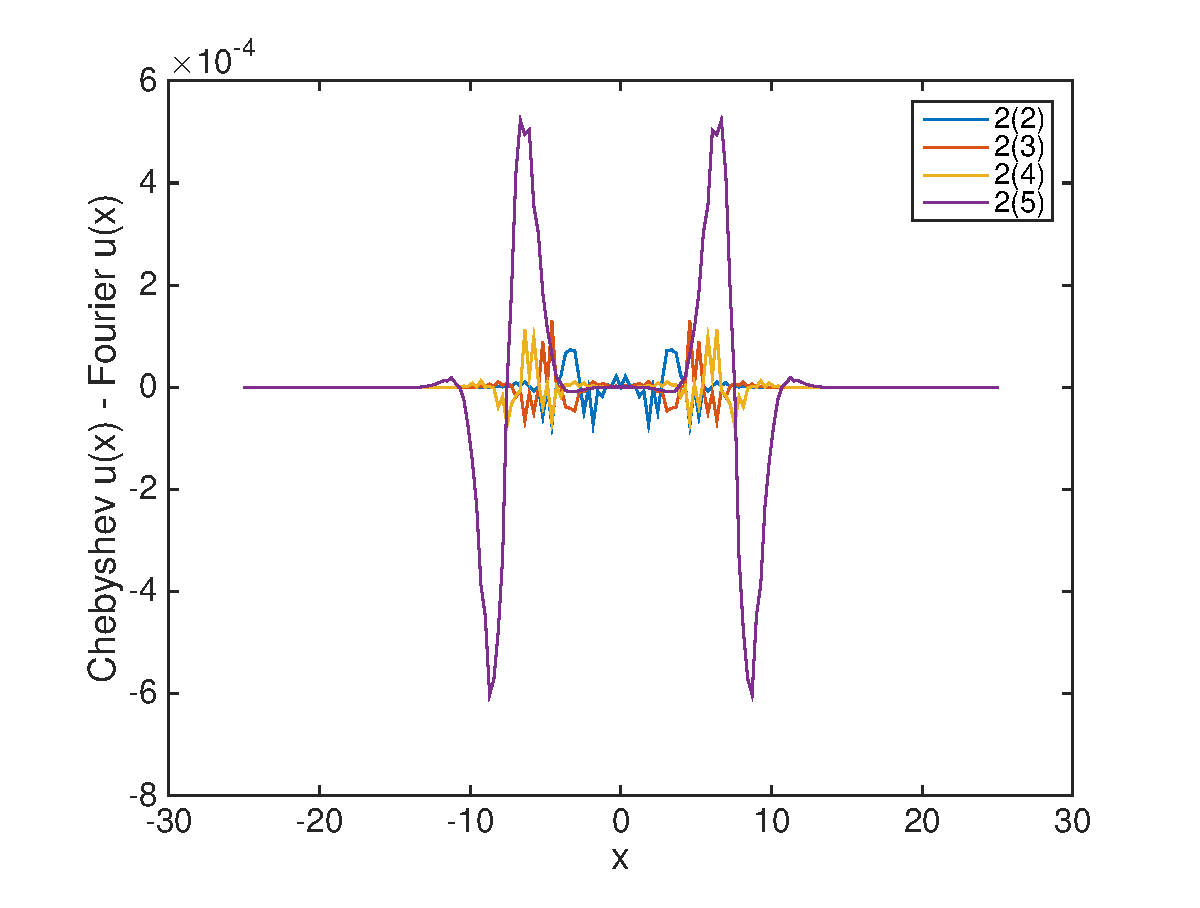
\includegraphics[width=8.5cm]{chebfourdiff.eps}
	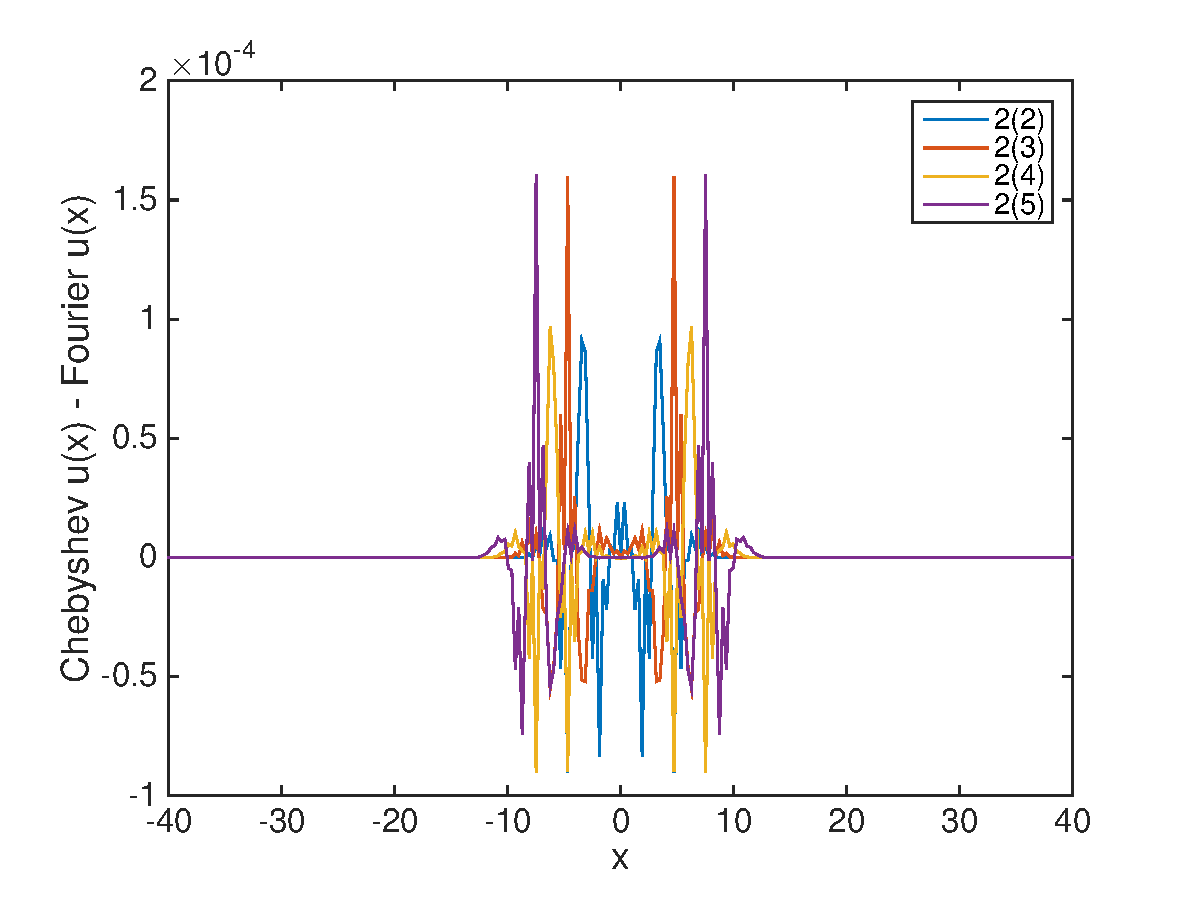
\includegraphics[width=8.5cm]{chebfourdiff40.eps}
	\caption{Difference between Chebyshev solution and Fourier solution for double pulses 2(2), 2(3), 2(4), and 2(5). Left is $N = 256$, domain size $L = 25$. Right is $N = 400$, domain size $L = 40$. Wave speed $c = 10$ for both cases.}
\end{figure}

\subsection{Eigenvalues and Eigenfunctions}

Next, we look at the two eigenvalue problems $Hv = \lambda v$ and $Lv = \lambda v$ corresponding to the linearization \eqref{linear4th} for the 4th order stationary equation \eqref{intKdV} and the linearization \eqref{linear5th} for the 5th order PDE \eqref{KdV5travel}, respectively. Since all our differential operators in Matlab are matrices, we can use the Matlab function \texttt{eig} to find these eigenvalues and eigenfunctions numerically. \\

First, we look at the eigenvalue problem $Hv = \lambda v$ posed on $L^2$ for the linearization \eqref{linear4th} of the 4th order stationary equation \eqref{intKdV}. For speed $c = 10$, we linearize about the single pulse and the first four double pulses. Since the operator $H$ is self-adjoint, the spectrum will be real. According to Theorem 2.3 in \cite{Pelinovsky2007}, for double pulses we should have a pair of eigenvalues near 0 and a pair of negative eigenvalues. The paired eigenvalue near 0 should switch signs with each subsequent double pulse. The table below shows that this is indeed the case.

\begin{table}[H]
\begin{tabular}{l|ll|ll}
Pulse  & Eigenvalue near 0  & Paired eigenvalue & Negative eigenvalue & Paired eigenvalue \\ \hline
1      & -5.5437e-12        &                   & -11.4747            &                   \\
2(1)   & 2.3172e-12         & -1.2782			& -11.5109            & -11.7293          \\
2(2)   & 3.6523e-12         & 0.0326            & -11.4720            & -11.4695          \\
2(3)   & -2.4674e-12        & -0.0008           & -11.4748            & -11.4748          \\
2(4)   & 2.3849e-12         & 2.0506e-05        & -11.4747            & -11.4747          \\
2(5)   & -2.4082e-12        & -7.1428e-07       & -11.4747            & -11.4747          \\
\end{tabular}
\caption{Eigenvalues of \eqref{linear4th}, the linearization of the 4th order stationary equation \eqref{intKdV} about single pulse 1 and double pulses 2(1), 2(2), 2(3), 2(4), and 2(5). Wave speed $c = 10$. Fourier spectral methods, $N = 256$.}
\end{table}

The absolute value of the paired eigenvalue near 0 decays exponentially, as we can see in the following figure. If we plot the absolute value of the eigenvalue vs the predicted distance between the pulses (normalized so that double pulse 2(2) has a distance of 0), the slope of the line is approximately $-\alpha$, as expected.
\begin{figure}[H]
	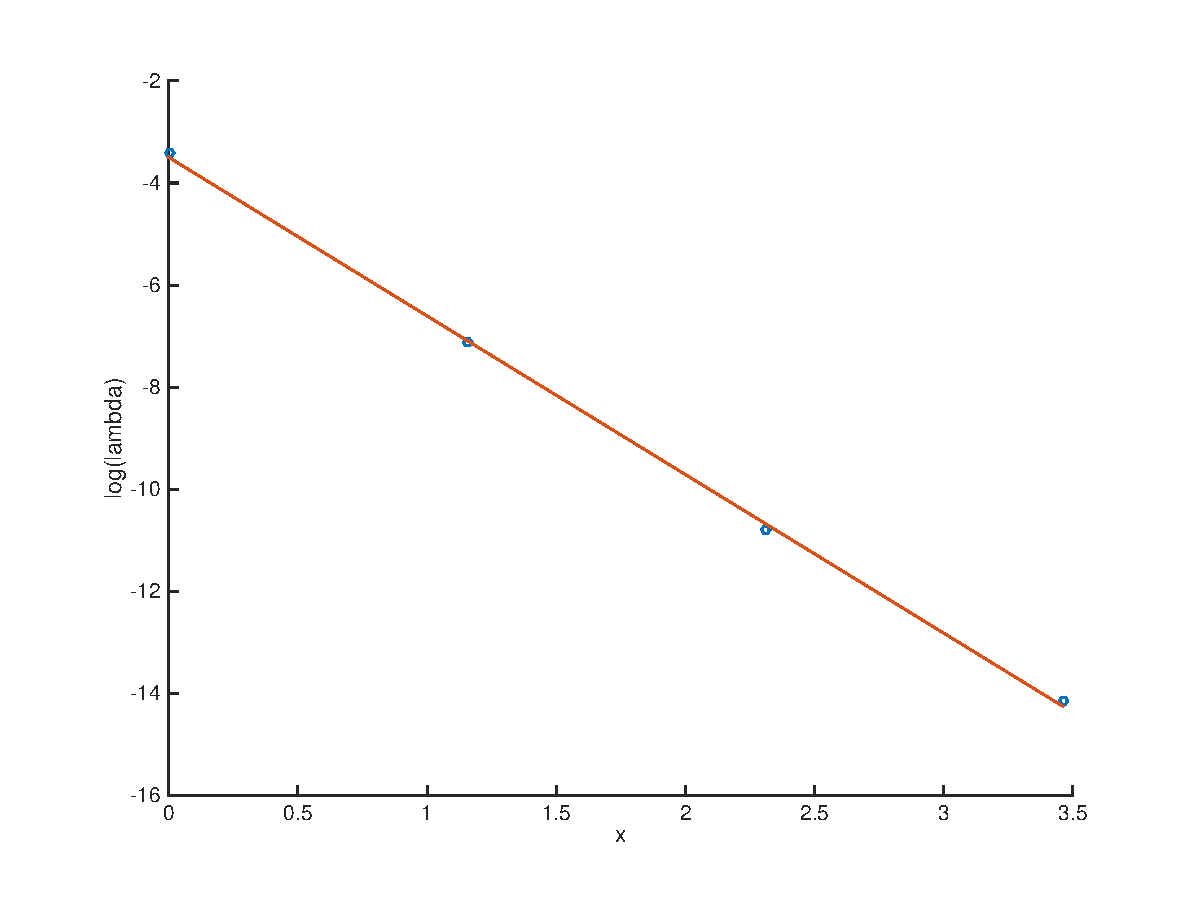
\includegraphics[width=8.5cm]{decayinteigenvalue}
	\caption{Exponential decay of absolute value of eigenvalue near 0 of \eqref{linear4th}, the linearization of the 4th order stationary equation \eqref{intKdV} about double pulses 2(2), 2(3), 2(4), and 2(5). The $x$-axis is predicted distance between the pulses, normalized so that double pulse 2(2) has a distance of 0. Wave speed $c = 10$, Fourier spectral methods, $N = 256$.}
\end{figure}

Next, we look at the eigenvalue problem $Lv = \lambda v$ posed on $L^2$ for the linearization \eqref{linear5th} of the 5th order PDE \eqref{KdV5travel}. For speed $c = 10$, we linearize about the first four double pulses.\\

First we do this using Fourier spectral methods (periodic boundary conditions). Here are plots of the spectra of the linearization about pulses 2(2) and 2(3).

\begin{figure}[H]
	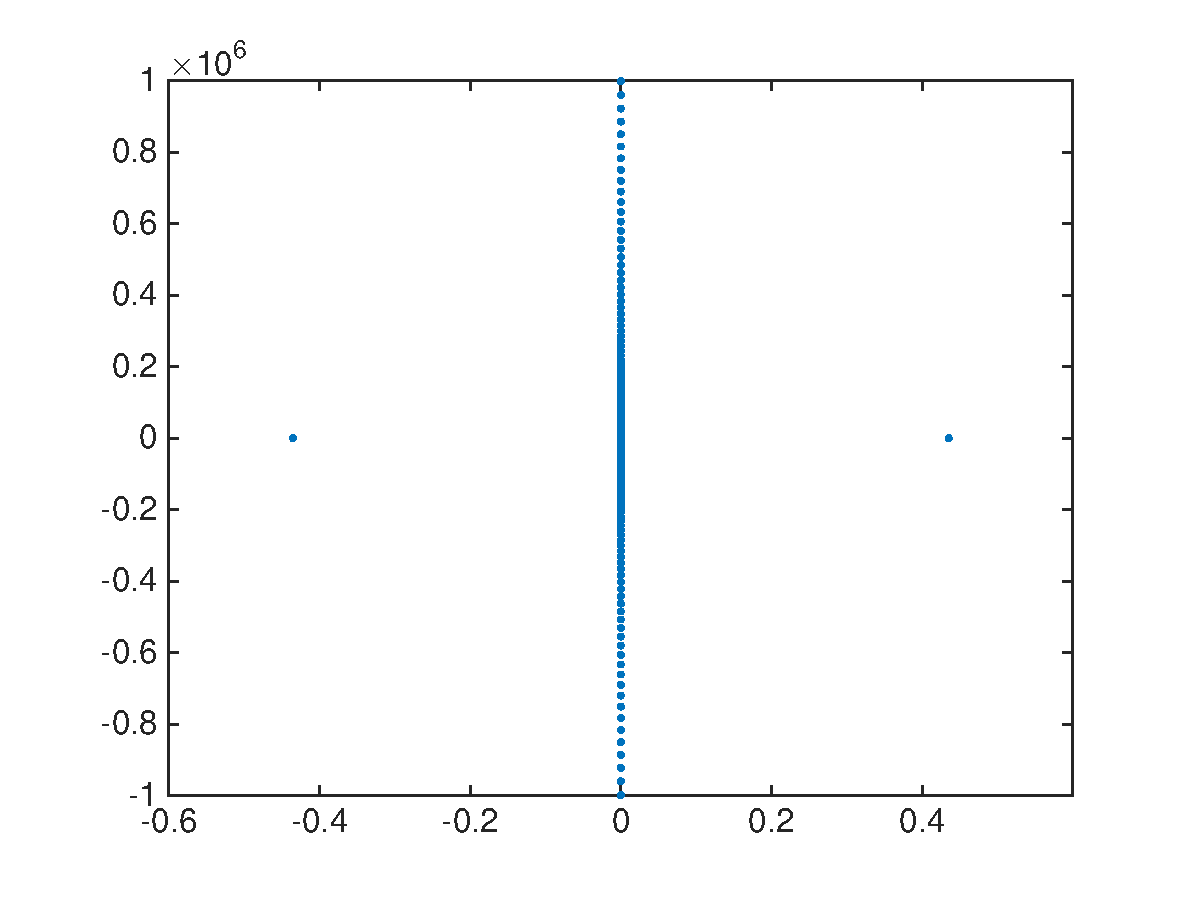
\includegraphics[width=8.5cm]{four10ud2_2}
	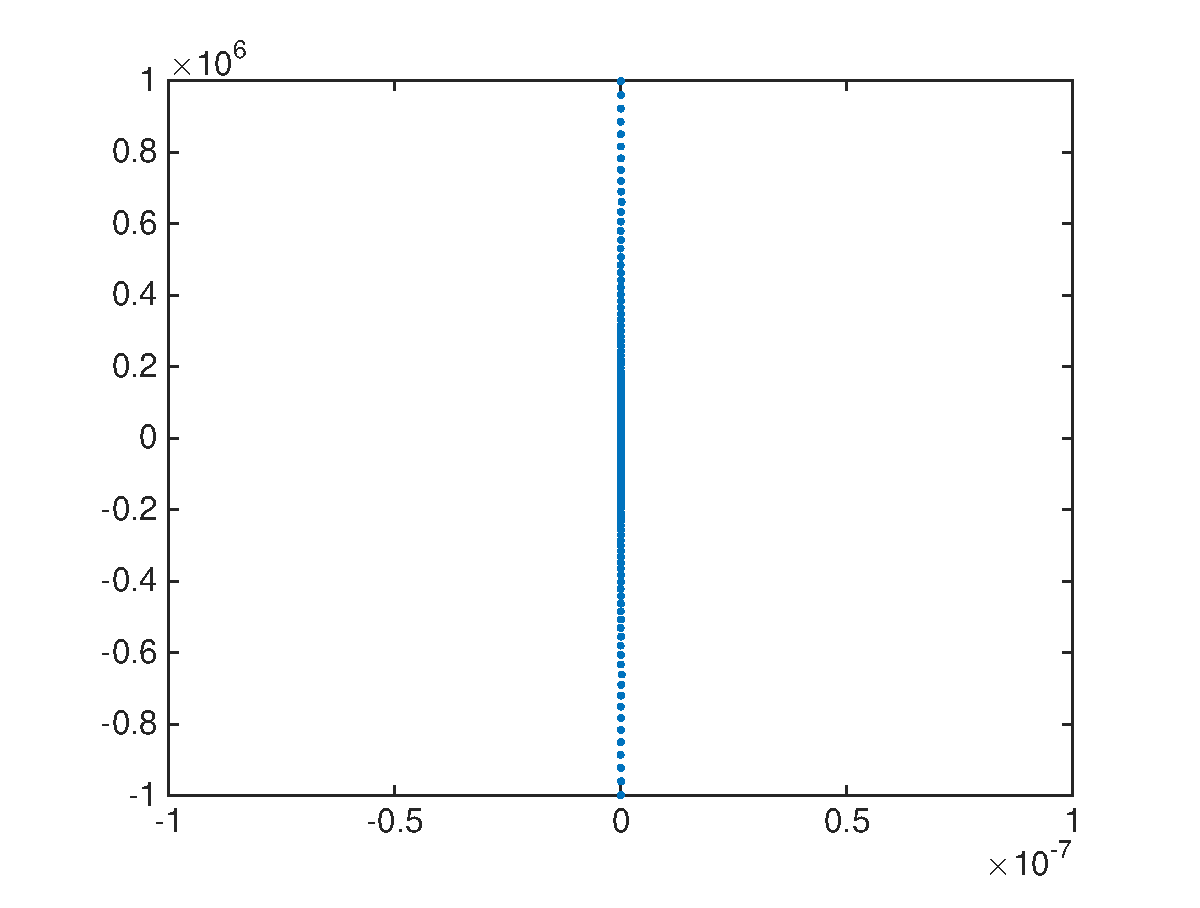
\includegraphics[width=8.5cm]{four10ud2_3}
	\caption{Spectrum of the linearization \eqref{linear5th} of the 5th order equation \eqref{KdV5travel} about double pulses 2(2) (left) and 2(3) (right). Wave speed $c = 10$, Fourier spectral methods, $N = 256$.}
\end{figure}

The essential spectrum for the 5th order equation is paramaterized by $ik(k^4 + k^2 + c), k \in \R$, which is the entire imaginary axis. In both cases, we see the essential spectrum on the imaginary axis, as expected. For double pulse 2(2), there is a pair of eigenvalues $\pm \lambda$ on the real axis.\\

For double pulse 2(3), no additional eigenvalues can be seen, so they must lie either on or close to the imaginary axis. To locate them, we shift to an exponentially weighted space. For an exponential weight $a$, we define the exponentially weighted spaces $L^2_a$ by

\begin{equation}\label{expweightedspace}
L^2_a = \{ f(x) : e^{ax} f(x) \in L^2\}
\end{equation}

In the exponentially weighted space $L^2_a$, the linear operator $L$ transforms to $e^{ax} L e^{-ax}$ \cite{Kapitula2013}. In essence, this involves replacing the differential operator $\partial_x$ with $(\partial_x - a)$. Thus the linearization \eqref{linear5th} of the 5th order equation \eqref{KdV5travel} about stationary solution $u^*(x)$ in the exponentially weighted space is

\begin{equation}\label{linear5thexpwt}
L_a = (\partial_x - a)^5 - (\partial_x - a)^3 + (c - 2 u^*)(\partial_x - a) - 2 u^*_x
\end{equation}

In the exponentially weighted space, the essential spectrum is paramaterized by the curve
\begin{align}\label{essentialspecexpwt}
(i k - a)^5 - (i k - a)^3 + c(i k - a) && k \in \R
\end{align}
The rightmost point of the essential spectrum occurs when $k = 0$, i.e. at the point $-a^5 + a^3 - c a$, which is always negative for $c > 1/4$ and $a > 0$. Since we are interested in wave speeds $c > 1/4$ and since we will be using a positive exponential weight, the essential spectrum will shift leftwards and will be separated from the imaginary axis.\\

In the next figure, we see the spectrum of the linearization of the 5th order equation about double pulse 2(3) in an exponentially weighted space with weight $a = 0.1$, i.e. the spectrum of the operator \eqref{linear5thexpwt} in $L^2_a$. The essential spectrum shifts to the left, as expected, and is very close to the essential spectrum predicted by \eqref{essentialspecexpwt}. Upon zooming in near the origin, we can also see a pair of complex-conjugate eigenvalues on (or very near) the imaginary axis.

\begin{figure}[H]
	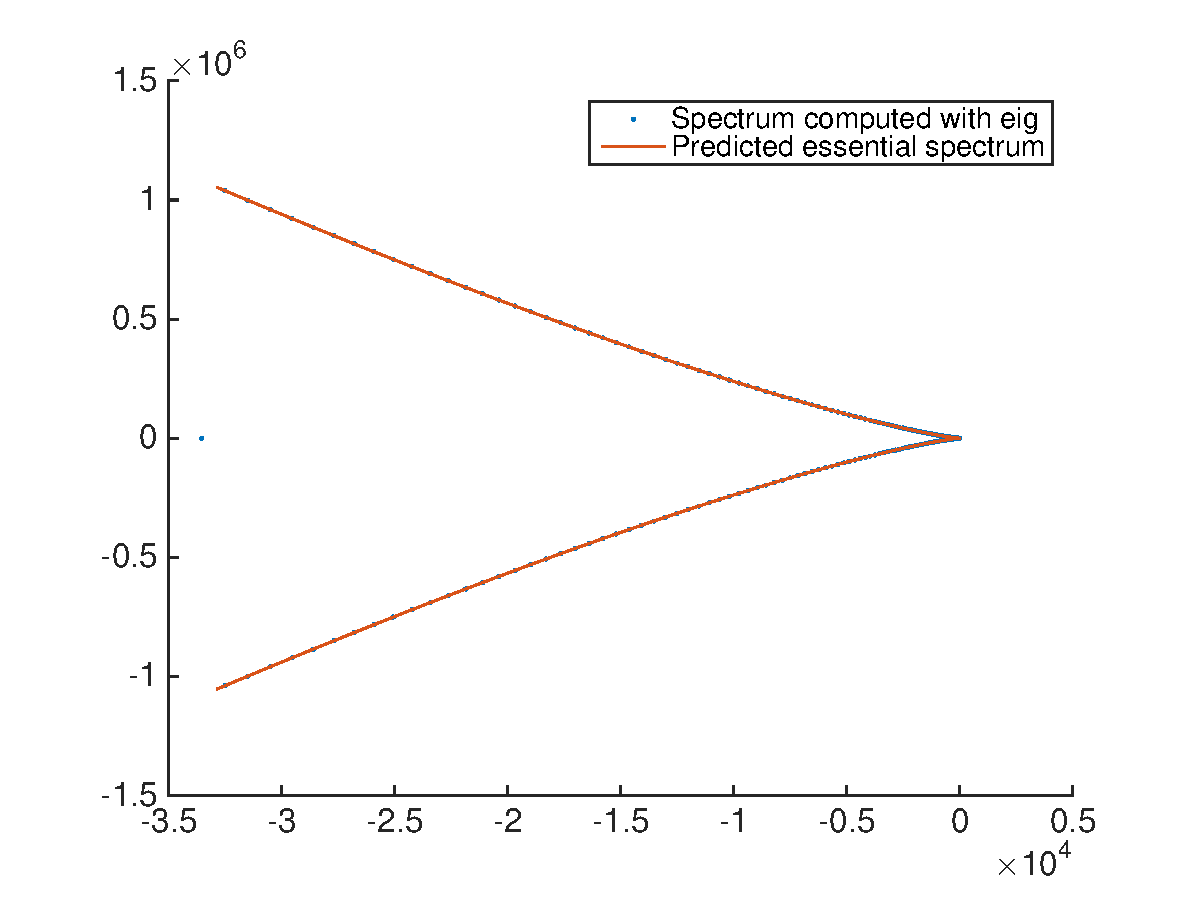
\includegraphics[width=8.5cm]{four10ud2_3expwt}
	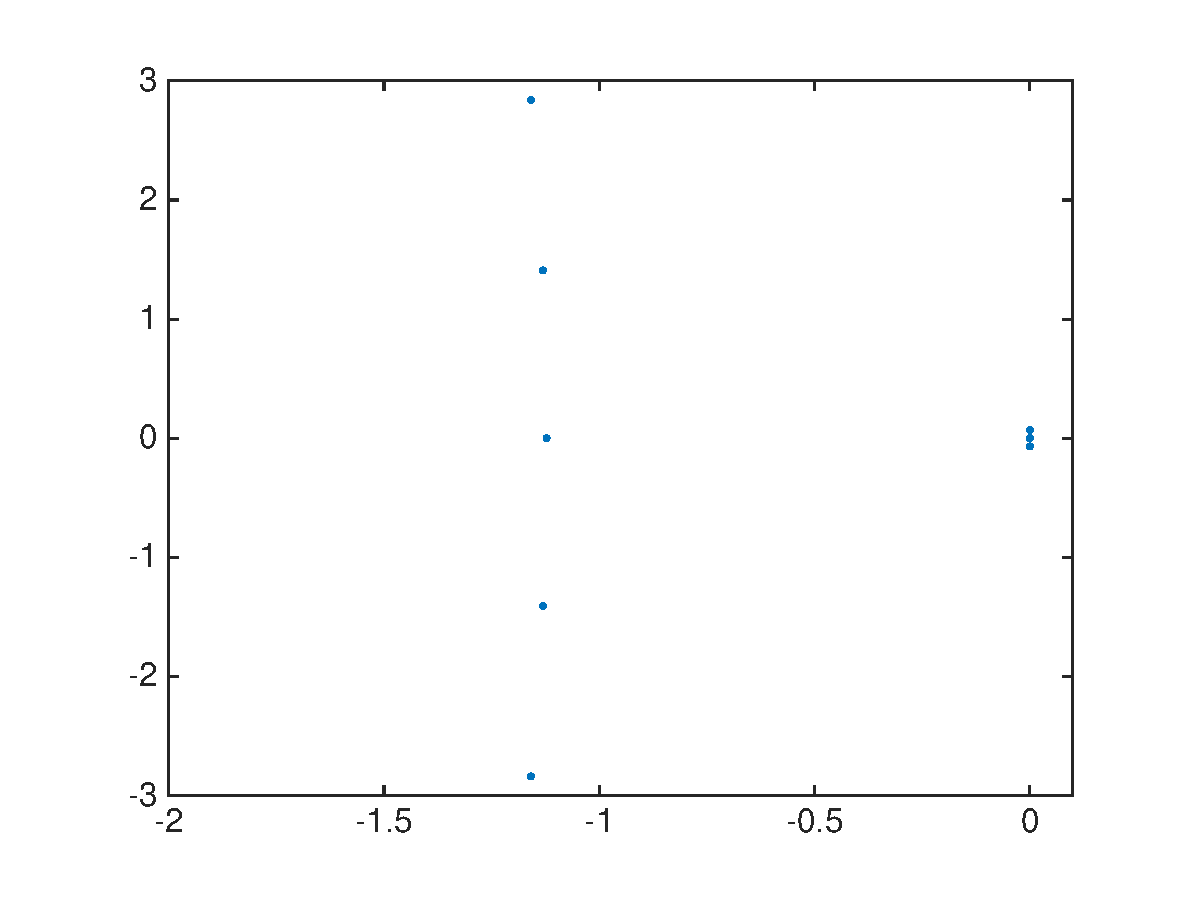
\includegraphics[width=8.5cm]{four10ud2_3expwt2}
	\caption{Spectrum of the linearization \eqref{linear5th} of the 5th order equation \eqref{KdV5travel} about double pulse 2(3) in exponentially weighted space with weight $a = 0.1$. Comparison with predicted essential spectrum is on left. Zoom around origin on right. Wave speed $c = 10$, Fourier spectral methods, $N = 256$.}
\end{figure}

Now that we have found the eigenvalues for double pulse 2(3) in the weighted space, we can locate them in the unweighted space since the point spectrum does not change when we apply an exponential weight. The figure below illustrates this.

\begin{figure}[H]
	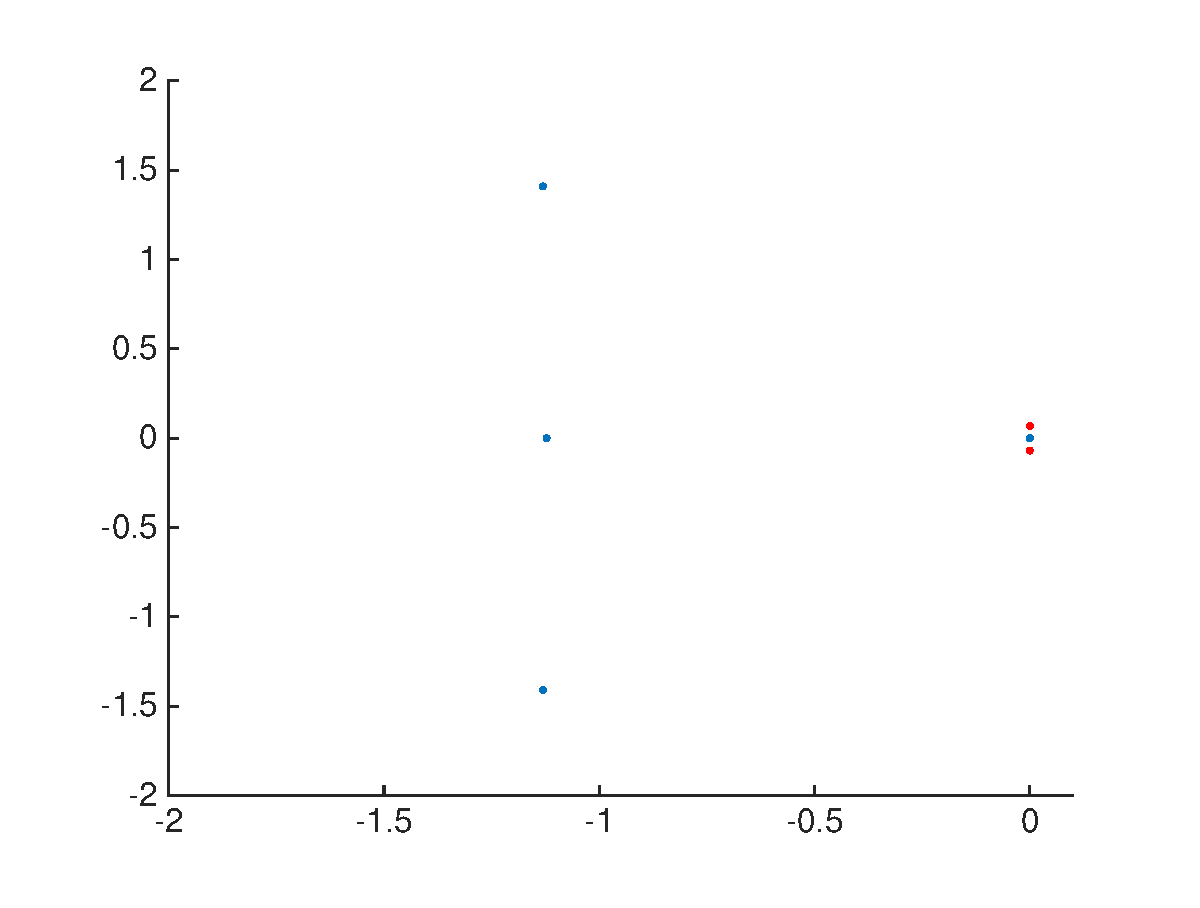
\includegraphics[width=8.5cm]{four10ud2_3redexpwt}
	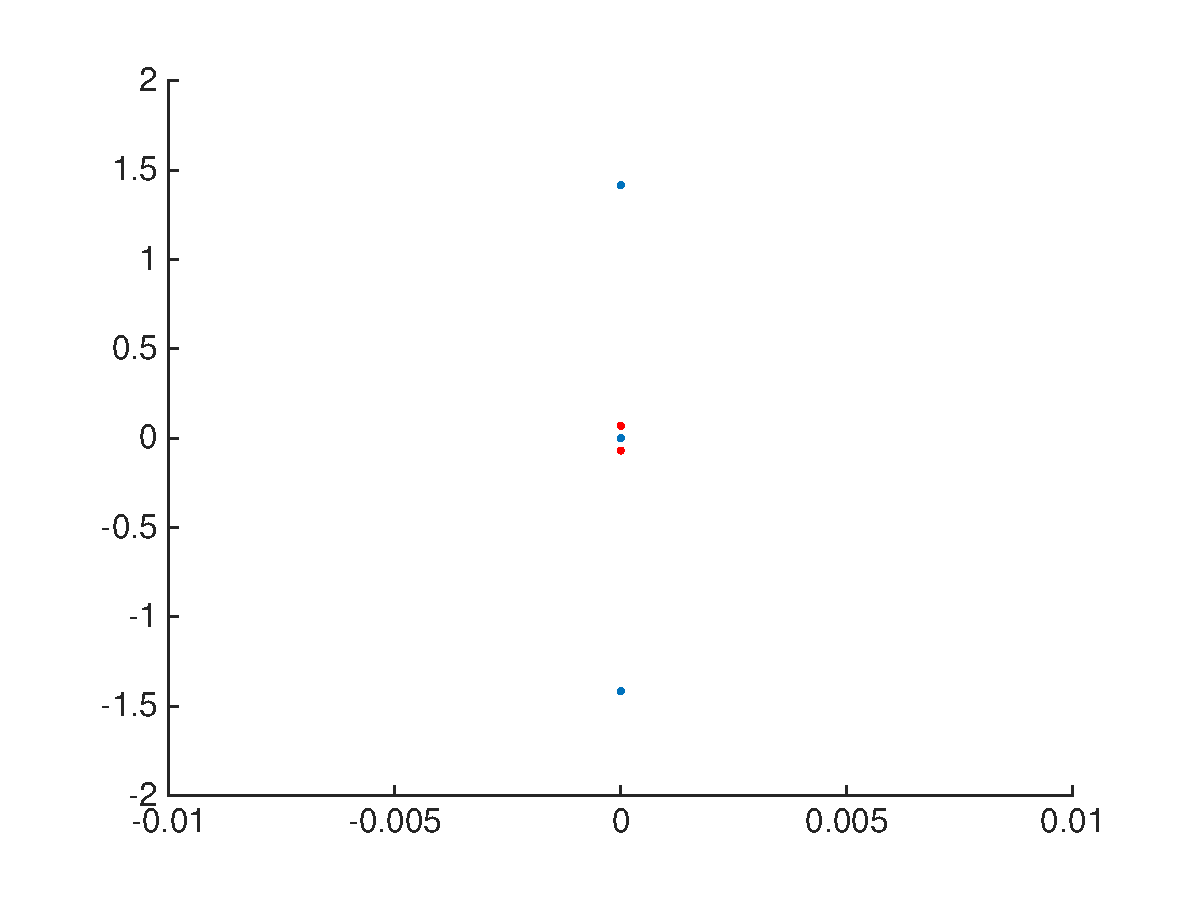
\includegraphics[width=8.5cm]{four10ud2_3red}
	\caption{On left, zoom around origin of spectrum of the linearization \eqref{linear5th} of the 5th order equation \eqref{KdV5travel} about double pulse 2(3) in exponentially weighted space with weight $a = 0.1$. Pair of nonzero, complex conjugate eigenvalues marked in red. On right, zoom around origin with same scaling on imaginary axis of spectrum of the linearization \eqref{linear5th} of the 5th order equation \eqref{KdV5travel} about double pulse 2(3) in unweighted space. The same eigenvalues we found in the weighted space are marked in red. Note that in both plots you can see points in the essential spectrum. For this discretization and boundary conditions, the eigenvalues have smaller absolute value than everything in the essential spectrum. Wave speed $c = 10$, Fourier spectral methods, $N = 256$.}
\end{figure}

Using Matlab's \texttt{eig} in the unweighted space, we can compute the nonzero eigenvalues of the linearization about the first four double pulses for speeds $c = 10, 7.5, 5$. The results of these computations are shown in the table below.

\begin{table}[H]
\begin{tabular}{l|lll}
 Double Pulse   & $c = 10$            & $c=7.5$                         & $c=5$        \\ \hline
  2(2) &     $\pm 0.4352$             & $\pm 0.2730$                    & $\pm 0.1363$ \\ 
  2(3) &     2.0829e-11 $\pm 0.0691i$ & -2.7698e-11 $\pm 0.0413i$       & 2.6806e-11 $\pm 0.0190i$\\ 
  2(4) &     $\pm 0.0109$             & $\pm 0.0062$                    & \\ 
  2(5) &    -8.5834e-13 $\pm 0.0020i$ & 6.8791e-12 $\pm$ 8.8812e-04$i$  & \\
\end{tabular}
\caption{Nonzero eigenvalues of \eqref{linear5th}, the linearization of 5th order PDE \eqref{KdV5travel} about double pulses 2(2), 2(3), 2(4), and 2(5) for wave speeds $c = 10, 7.5, 5$. Fourier spectral methods, $N = 256$}
\end{table}

For double pulses 2(3) and 2(5), there is a pair of complex conjugate eigenvalues which are very near to the imaginary axis. We would like to know if the real part is numerical error, i.e. if the real part is actually 0. Three pieces of numerical evidence suggest that this is actually the case. First, the sign of the small real part is not consistent, i.e. there seems to be no pattern as to whether it is positive or negative. Second, it is not hard to show that if $a + bi$ is an eigenvalue, then so is $-a + bi$. Thus if the real part is nonzero, we should expect a quartet of nonzero eigenvalues rather than a pair like we observe. Finally, we can use Matlab's \texttt{fsolve} command to eliminate the small real part and obtain a ``better'' eigenfunction, i.e. one for which $\max{|Jv - \lambda v|}$ is smaller, where $J$ is the linearization about the double pulse. To do this, we note that since $J$ is real, if we have a purely imaginary eigenvalue $\lambda = \gamma i$ with corresponding eigenfunction $v(x) = w_1(x) + i w_2(x)$, then we can write the eigenvalue problem as the pair of real-valued equations

\begin{align}\label{realeigproblem}
Jw_1 &= -\gamma w_2 \\
Jw_2 &= \gamma w_1
\end{align}

The output of \texttt{eig} is the eigenvalues $\lambda$ and eigenfunction $v(x) = w_1(x) + i w_2(x)$. Using $w_1(x)$, $w_2(x)$, and $\gamma = \textrm{Re} \lambda$ as our initial guess, we use \texttt{fsolve} on $[w_1(x); w_2(x); \gamma]$ to construct a new eigenfunction / eigenvalue pair (the eigenvalue changes by only a tiny amount). This new pair is ``better'' in the sense that $\max{|Jv - \lambda v|}$ is smaller. Details are given in the table below.

\begin{table}[H]
\begin{tabular}{l|ll}
 Double Pulse   & $\max{|Lv - \lambda v|}$ before \texttt{fsolve} & $\max{|Lv - \lambda v|}$ after \texttt{fsolve}\\ \hline
  2(3) & 4.4440e-11 & 7.2469e-12 \\
  2(5) & 5.3975e-11 & 5.5005e-12 \\
\end{tabular}
\caption{Maximum of eigenvalue problem $|Lv - \lambda v|$ before and after using Matlab's \texttt{fsolve} to eliminate small real part of eigenvalue. Wave speed $c = 10$, Fourier spectral methods, $N = 256$.}
\end{table}


Now we take a look at the eigenfunctions. For the eigenfunctions with real eigenvalue, i.e. for double pulses 2(2) and 2(4), we have the following eigenfunctions.

\begin{figure}[H]
	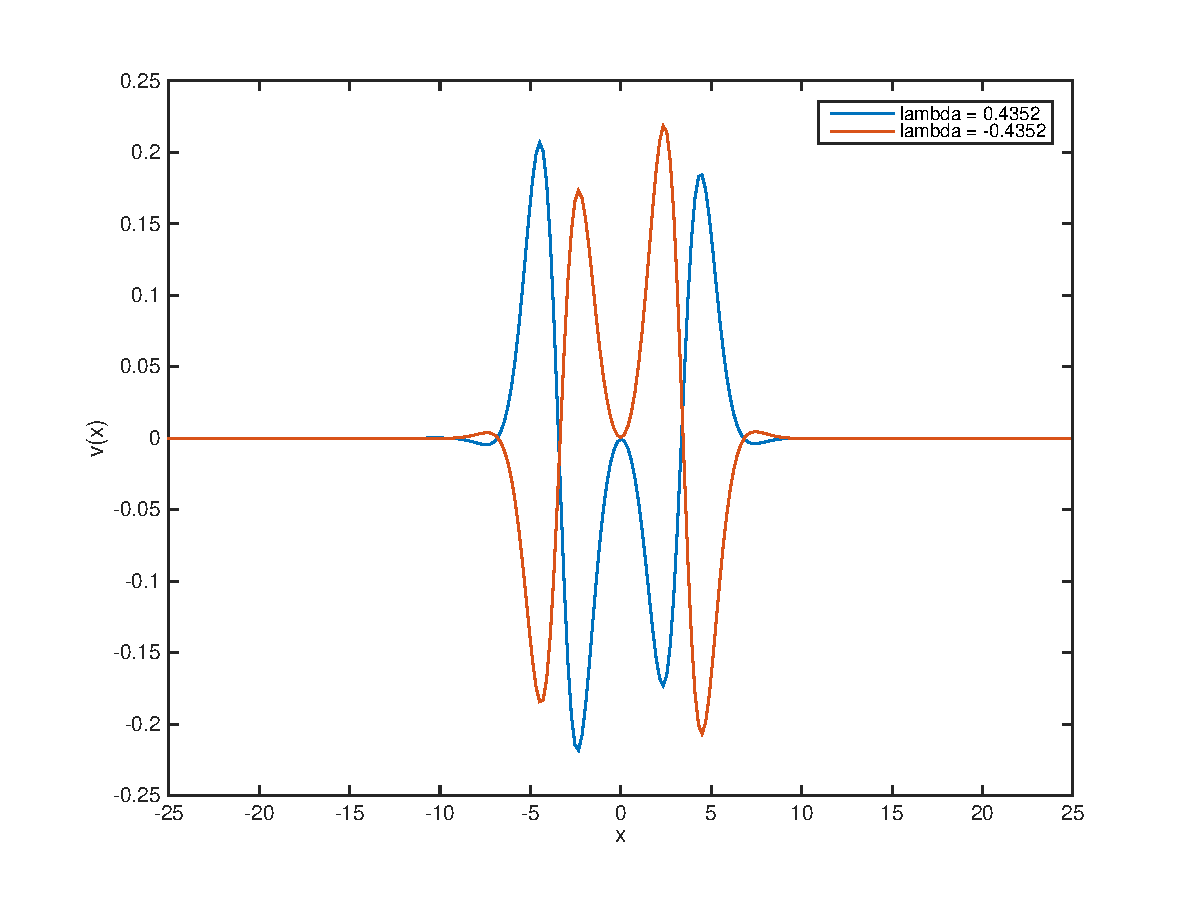
\includegraphics[width=8.5cm]{four10dp1eigenfns}
	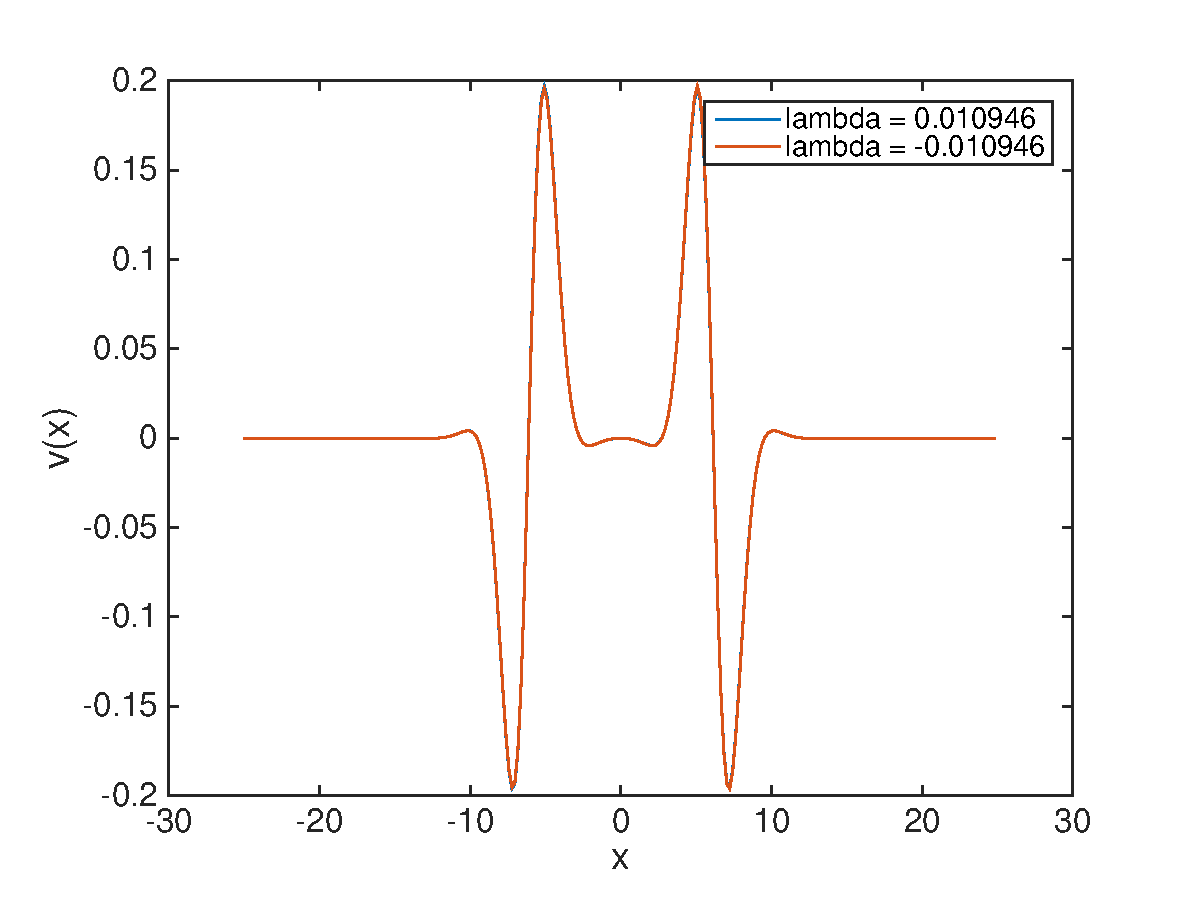
\includegraphics[width=8.5cm]{four10dp3eigenfns}
	\caption{Eigenfunctions corresponding to eigenvalues for linearization \eqref{linear5th} of 5th order PDE \eqref{KdV5travel} about double pulses 2(3) and 2(5). Wave speed $c = 10$, Fourier spectral methods, $N = 256$}
\end{figure}

As we did with the single pulses, we can look at the exponential decay rates of the eigenfunctions. The characteristic polynomial in this case is 

\begin{equation} \label{charpoly2}
\nu^5 - \nu^3 + c \nu - \lambda = 0
\end{equation}

For double pulse 2(2) with $c = 10$, we have eigenvalue $0.4352$, the complex roots of the characteristic polynomial \eqref{charpoly2} are $-1.3639 \pm 1.1556i, 1.3422 \pm 1.1521i$. The exponential decay rate is close to the real part of these roots, as we see in the plot below.

\begin{figure}[H]
	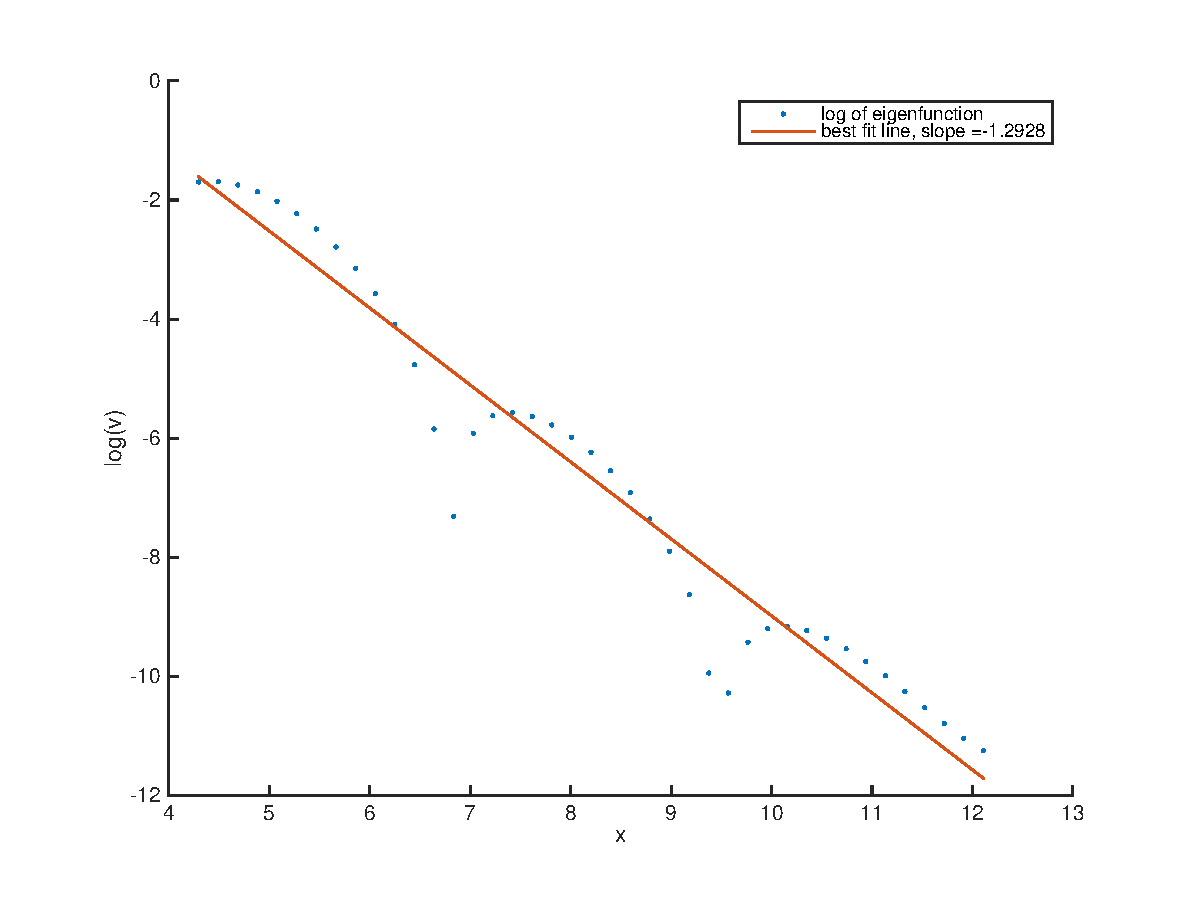
\includegraphics[width=8.5cm]{decayeigenfunction}
	\caption{Plot of $\log v(x)$ vs $x$ for eigenfunction $v(x)$ of linearization \eqref{linear5th} of 5th order PDE \eqref{KdV5travel} about double pulse 2(2). Eigenfunction $v(x)$ corresponding to positive eigenvalue ($\lambda = 0.4352$) is chosen. Slope of best fit line on left is -1.2928, which is close to the real parts of the roots of the characteristic polynomial for the eigenvalue problem. Wave speed $c = 10$, Fourier spectral methods, $N = 256$.}
\end{figure}

We can also look at the integral of the eigenfunctions. We expect the integral of each eigenfunction to be 0. Using the discrete integral for an evenly-spaced grid, we see that this is approximately the case.

\begin{table}[H]
\begin{tabular}{l|l}
Pulse  & Integral of eigenfunction \\ \hline
2(2)   & -3.5238e-11   \\
2(3)   & -4.7037e-12 - 2.0787e-10i  \\
2(4)   & 1.3412e-09  \\
2(5)   & -1.7373e-11 - 1.7818e-08i  \\
\end{tabular}
\caption{Integral of eigenfunctions corresponding to eigenvalues near 0 for linearization \eqref{linear5th} of 5th order PDE \eqref{KdV5travel} about double pulses 2(2), 2(3), 2(4), and 2(5). We take eigenfunction corresponding to positive eigenvalue (double pulses 2(2) and 2(4)) or eigenvalue with positive imaginary part (double pulses 2(3) and 2(5)). Wave speed $c = 10$, Fourier spectral methods, $N = 256$.}
\end{table}

Now we take a look at the eigenfunctions corresponding to double pulse 2(3), i.e. eigenvalues which are purely imaginary (at least to leading order). Plots of the real and imaginary part of these eigenfunctions are give below.

\begin{figure}[H]
	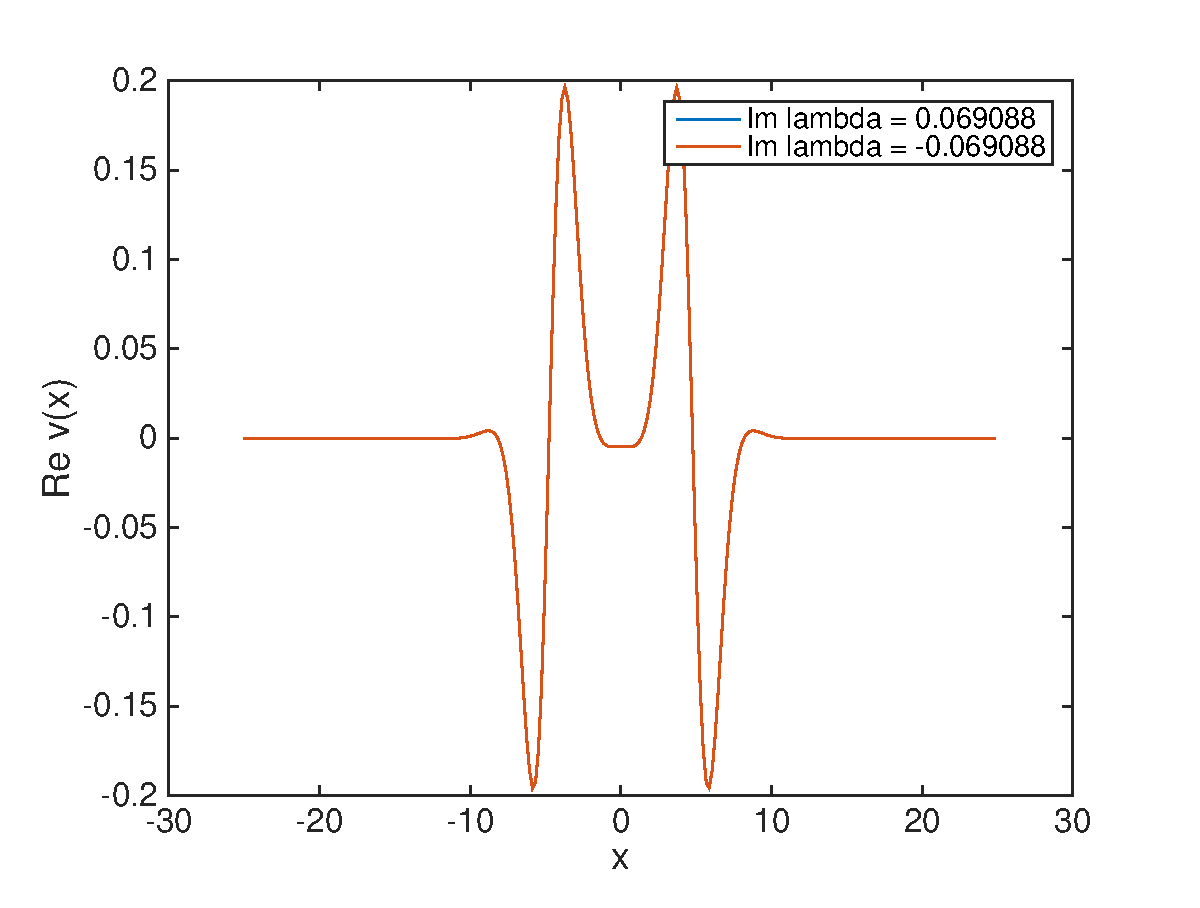
\includegraphics[width=8.5cm]{four10dp2eigenfnsreal}
	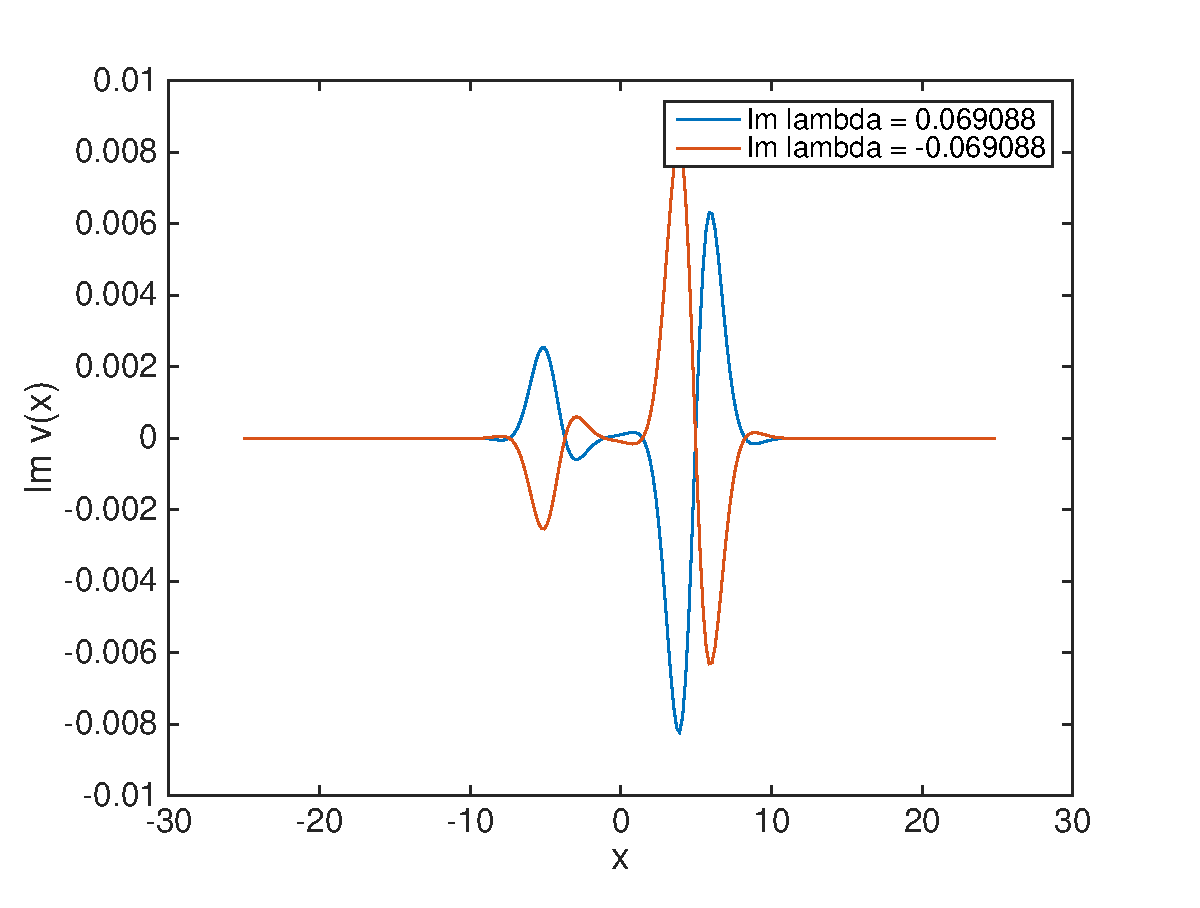
\includegraphics[width=8.5cm]{four10dp2eigenfnsimag}
	\caption{Real (left) and imaginary (right) parts of eigenfunctions corresponding to eigenvalues for linearization \eqref{linear5th} of 5th order PDE \eqref{KdV5travel} about double pulse 2(3). Wave speed $c = 10$, Fourier spectral methods, $N = 256$.}
\end{figure}

Since eigenfunctions are only specified up to a constant multiple, for a purely imaginary eigenvalue $\lambda = \beta i$ and corresponding eigenfunction $v(x)$, it is not hard to show that we can find an angle $\theta$ such that the rotated eigenfunction $\tilde{v}(x) = e^{i \theta} v(x)$ has even real part and odd imaginary part. If we use \texttt{fsolve} to eliminate the small real part (as we did above), we can then find an angle of rotation to accomplish this. Plots of these modified eigenfunctions are shown below.

\begin{figure}[H]
	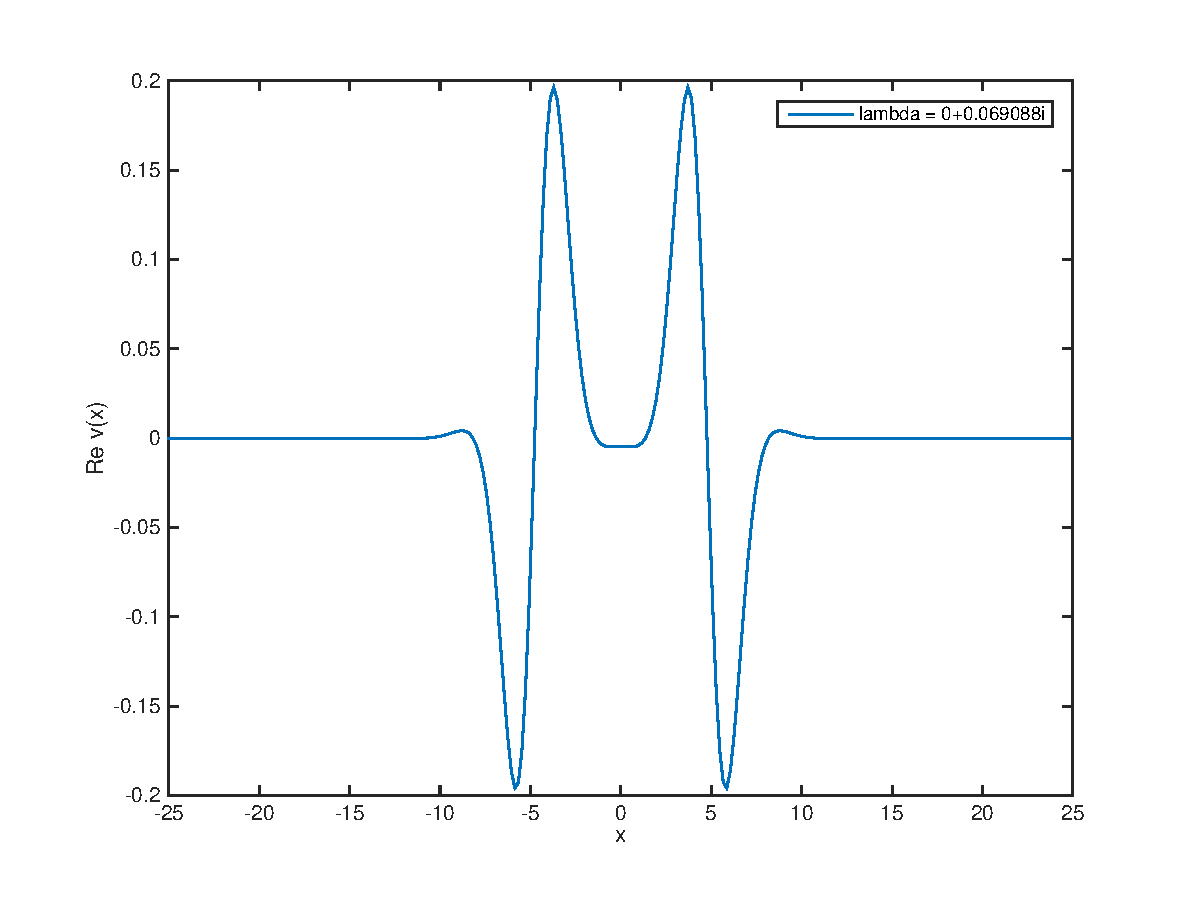
\includegraphics[width=8.5cm]{four10dp2eigenfnsreal_after}
	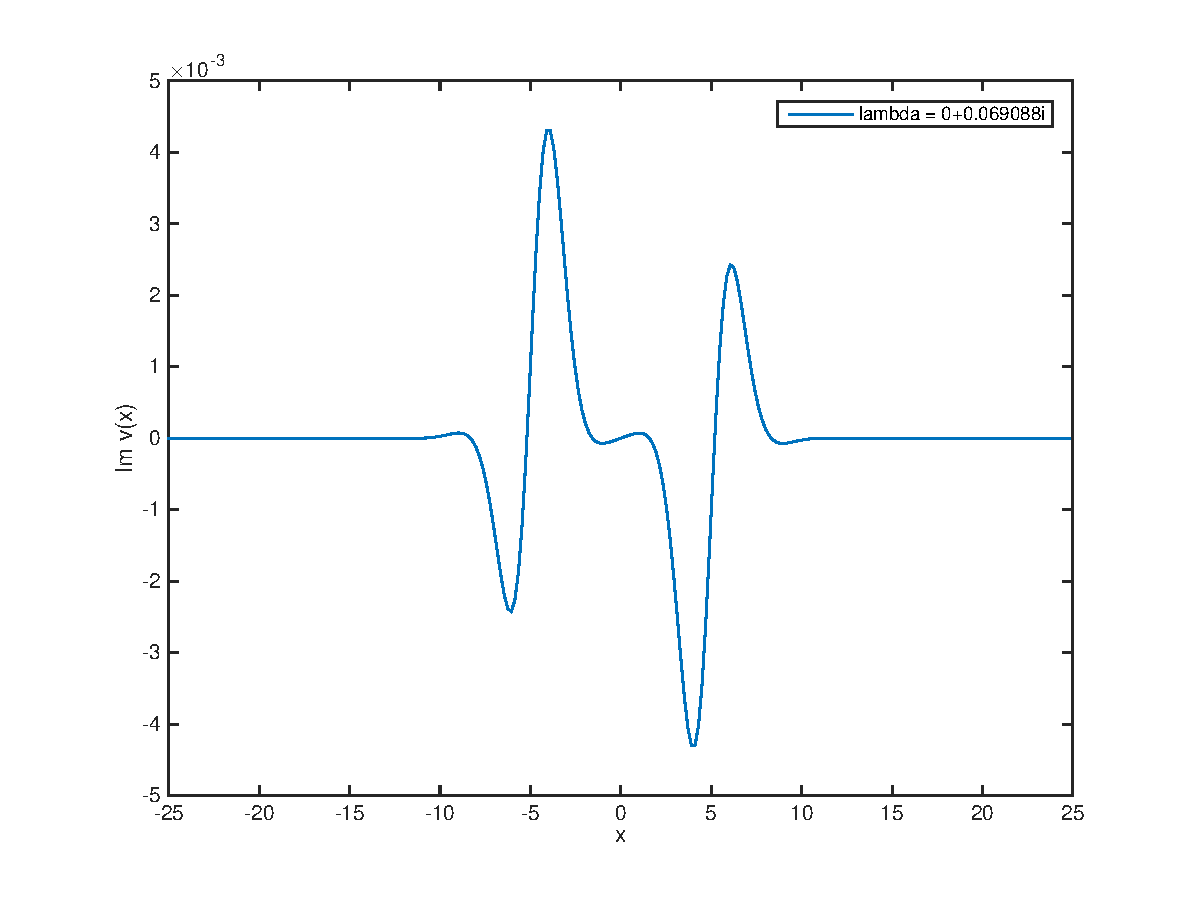
\includegraphics[width=8.5cm]{four10dp2eigenfnsimag_after}
	\caption{Real (left) and imaginary (right) parts of eigenfunctions corresponding to eigenvalue with positive imaginary part for linearization \eqref{linear5th} of 5th order PDE \eqref{KdV5travel} about double pulse 2(3) after elimination of small real part of eigenvalue using \texttt{fsolve} and rotation by unit complex number. Wave speed $c = 10$, Fourier spectral methods, $N = 256$.}
\end{figure}

Just as we did with the eigenvalues of the 4th order ODE \eqref{intKdV}, we can show that the absolute value of the eigenvalues of the 5th order equation \eqref{KdV5travel} decay exponentially. We can actually predict these eigenvalues! Consider the second order system

\begin{align}\label{simplesystem}
\dot{x} &= y \\
\dot{y} &= C^2 e^{-\alpha x} \sin{\beta x}
\end{align}

where $\alpha$ and $\beta$ are the real and imaginary parts of the roots of the characteristic polynomial \eqref{charpoly1} and $C$ is a constant. This system has equilibria at $(n \pi / \beta, 0), n \in \Z$. For $n$ even, the eigenvalues for the linearization about the equilibria are $\lambda = \pm C \sqrt{\beta}\exp{(-\alpha n \pi / 2 \beta)}$ (saddle point), and for $n$ odd, the eigenvalues are $\lambda = \pm i C \sqrt{\beta}\exp{(-\alpha n \pi / 2 \beta)}$ (center). If we choose $C$ such that the eigenvalue for $n = 0$ corresponds to the eigenvalue for double pulse 2(2), we get a very good prediction for the eigenvalues of the linearization about the double pulses. This is shown in the figure below.

\begin{figure}[H]
	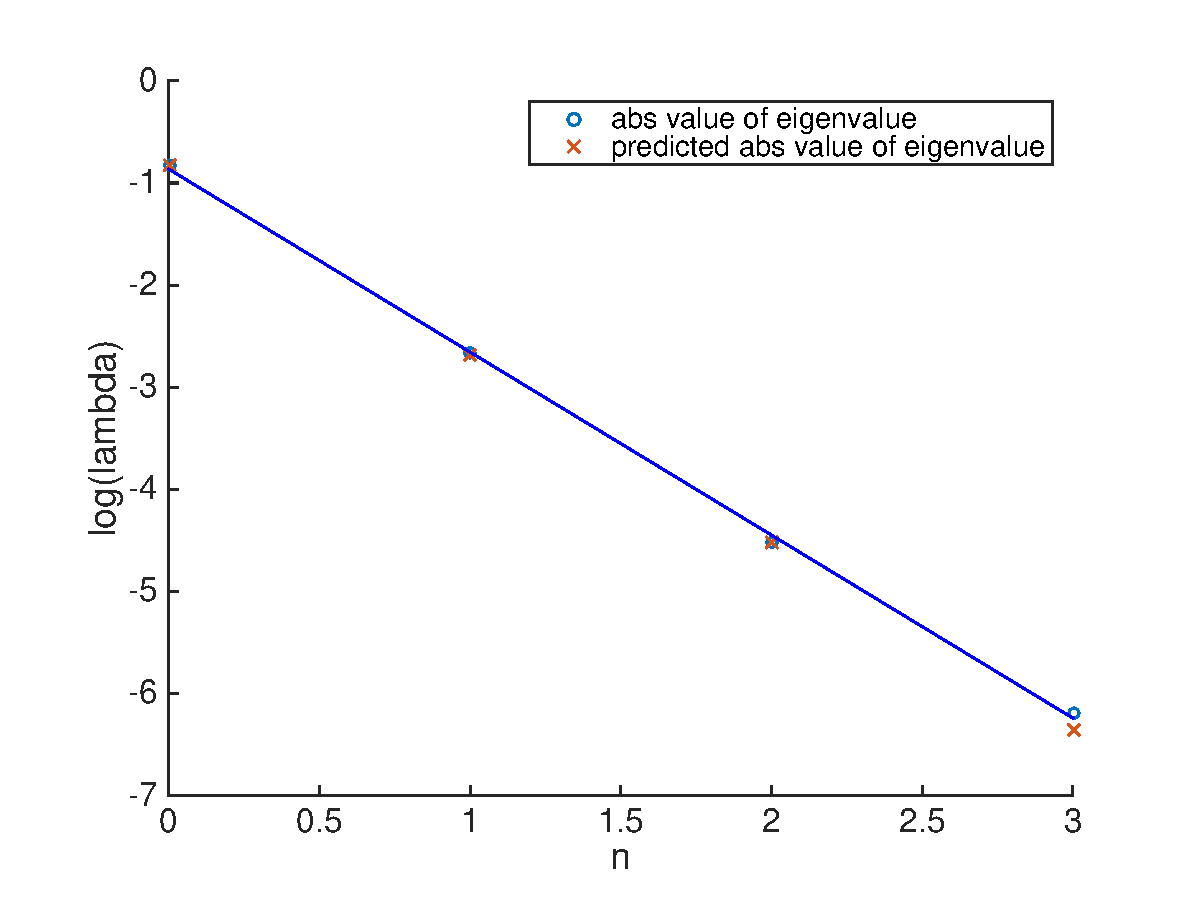
\includegraphics[width=8.5cm]{decayeigenvalue}
	\caption{Exponential decay of absolute value of eigenvalues of linearization \eqref{linear5th} of 5th order PDE \eqref{KdV5travel} about double pulse solutions. Plot also shows the predicted values of the absolute value of the eigenvalues, using formula $|\lambda| = C \sqrt{\beta}\exp{(-\alpha n \pi / 2 \beta)}$, where $C$ is a constant chosen as described above. Waves are 2(2), 2(3), 2(4), and 2(5); these correspond to $n = 0, 1, 2, 3$ in the formula. Wave speed $c = 10$, Fourier spectral methods, $N = 256$.}
\end{figure}

Finally, we can look at the essential spectrum as the domain length $L$ increases. We require more Fourier nodes $N = 768$) to do this to ensure that enough grid points capture the wave in the center. The next plot shows the imaginary part of the spectrum for domain lengths from 25 to 165. The two nonzero eigenvalues on (or near) the imaginary axis are shown in red; these remain stationary as the domain length increases. As $L$ increases, the other points on the essential spectrum move down the imaginary axis towards the origin. However (at least for the values of $L$ we looked at here), these essential spectrum points always remain further from the origin than the two nonzero eigenvalues. They never ``cross over'' the eigenvalues.

\begin{figure}[H]
	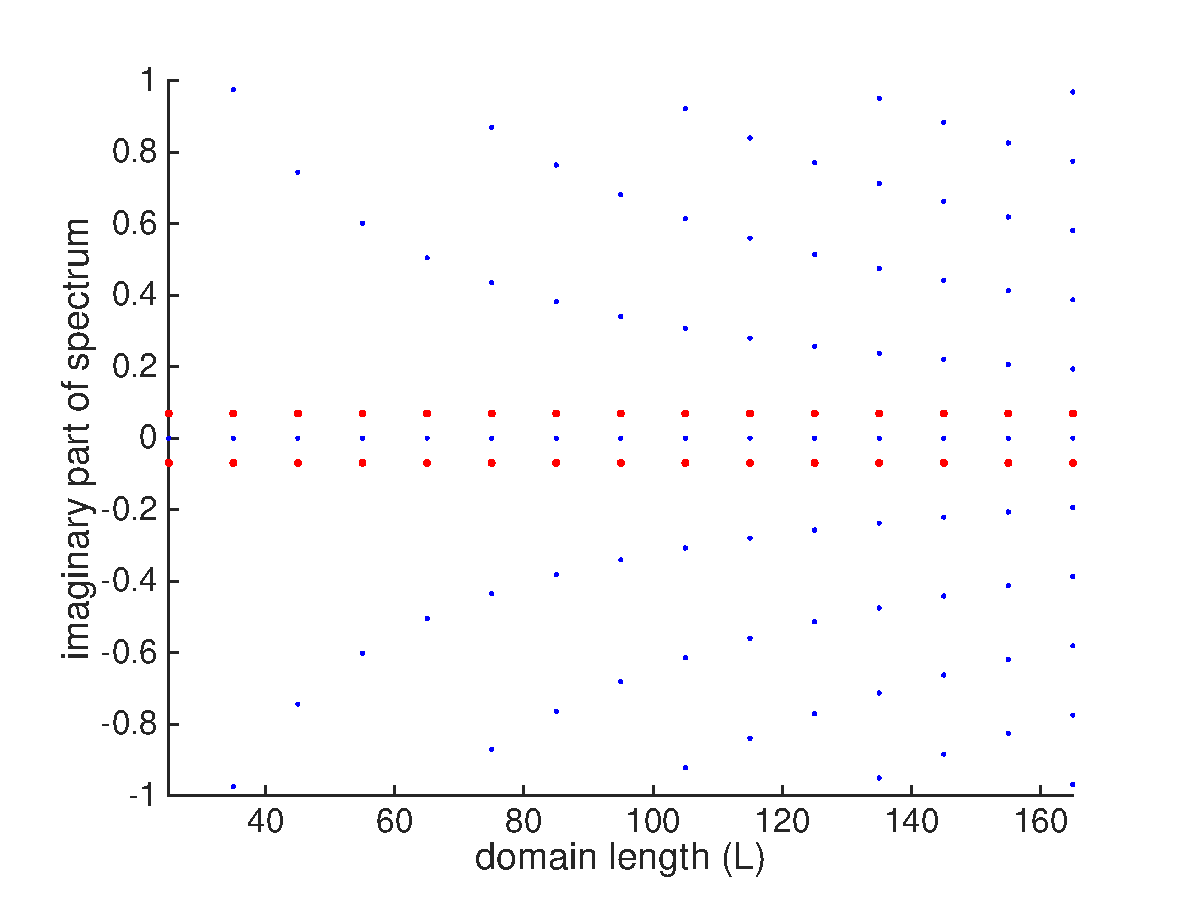
\includegraphics[width=8.5cm]{essspecL}
	\caption{Imaginary part of the spectrum of the linearization \eqref{linear5th} of 5th order PDE \eqref{KdV5travel} about double pulse 2(2) plotted for domain lengths $L$ from 25 to 165. Imaginary part of nonzero eigenvalues are shown in red. Wave speed $c = 10$, Fourier spectral methods, $N = 768$.}
\end{figure}

We can also look at the nonzero eigenvalues as a function of domain length.

\begin{table}[H]
\begin{tabular}{l|l}
Domain Length (L)  & Nonzero eigenvalues \\ \hline
    25 &  $  2.3036e-09 \pm 0.0691i$   \\
    35 &  $  5.6015e-11 \pm 0.0691i$   \\
    45 &  $  1.4699e-10 \pm 0.0691i$   \\
    55 &  $ -2.6976e-11 \pm 0.0691i$   \\
    65 &  $  1.1296e-11 \pm 0.0691i$   \\
    75 &  $  5.1110e-12 \pm 0.0691i$   \\
    85 &  $ -4.4132e-12 \pm 0.0691i$   \\
    95 &  $  2.6624e-12 \pm 0.0691i$   \\
   105 &  $  2.3847e-12 \pm 0.0691i$   \\
   115 &  $ -1.1708e-12 \pm 0.0691i$   \\
   125 &  $  3.0109e-13 \pm 0.0691i$   \\
   135 &  $ -3.4430e-13 \pm 0.0691i$   \\
   145 &  $  1.0531e-12 \pm 0.0691i$   \\
   155 &  $  5.5331e-14 \pm 0.0691i$   \\
   165 &  $  4.2756e-13 \pm 0.0691i$   \\
\end{tabular}
\caption{Nonzero eigenvalues of linearization \eqref{linear5th} of 5th order PDE \eqref{KdV5travel} about double pulse 2(2) for domain lengths from 25 to 165. Wave speed $c = 10$, Fourier spectral methods, $N = 768$.}
\end{table}

Plotting the log of the real part of the nonzero eigenvalue versus domain length, we have a reasonable linear fit, which suggests that the real part of the nonzero eigenvalue decays exponentially as the domain length $L$ increases.

\begin{figure}[H]
	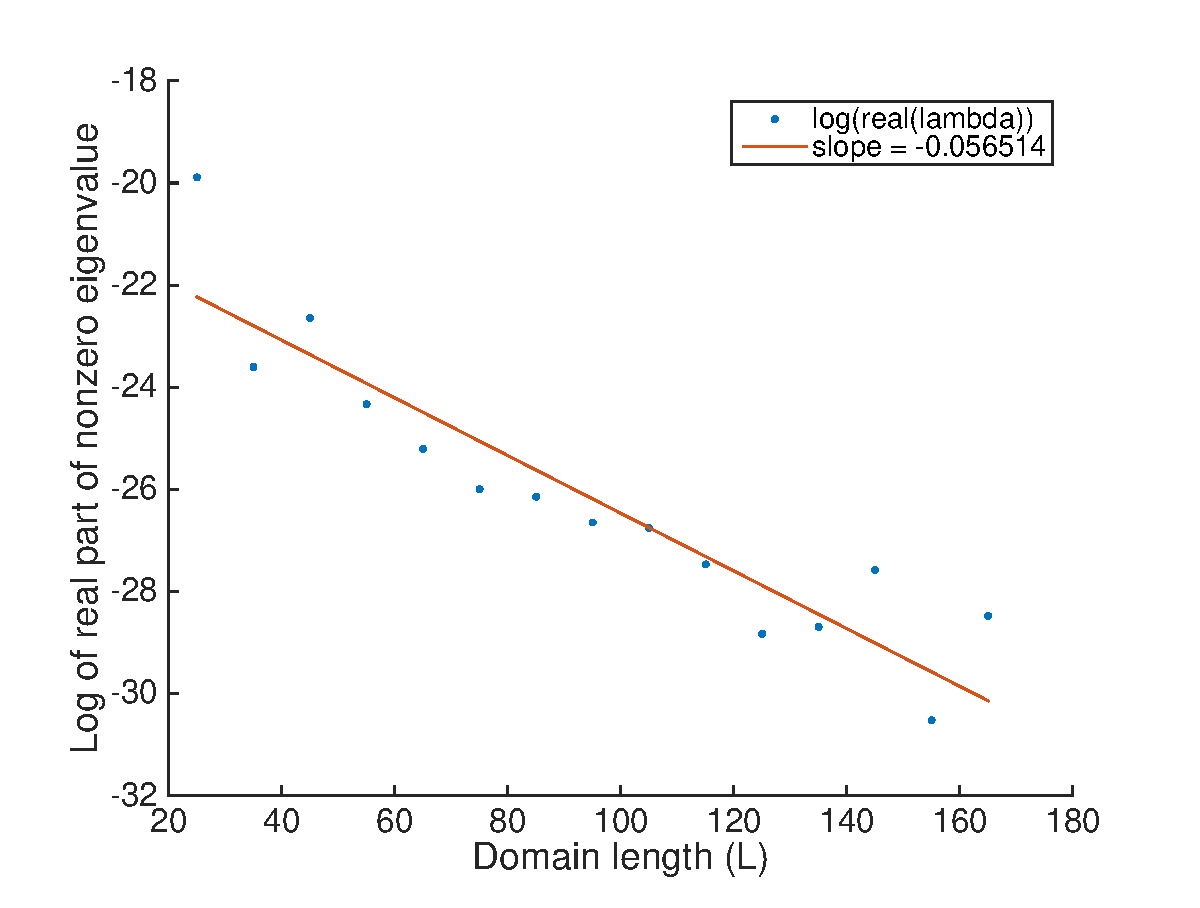
\includegraphics[width=8.5cm]{expdecayL}
	\caption{Plot of the log of the real part of the nonzero eigenvalues of the linearization \eqref{linear5th} of 5th order PDE \eqref{KdV5travel} about double pulse 2(2) versus domain length $L$. Wave speed $c = 10$, Fourier spectral methods, $N = 768$.}
\end{figure}


We repeat the above using Chebyshev spectral methods. Since we are using separated boundary conditions on a finite domain, we no longer see the essential spectrum. Instead, we see the absolute spectrum. (I SHOULD LOOK INTO THIS MORE; FOR EXAMPLE, I COULD COMPUTE THE ABSOLUTE SPECTRUM NUMERICALLY AND COMPARE IT TO THE PLOTS.) For the linearization about double pulse 2(2), we have the following spectrum.

\begin{figure}[H]
	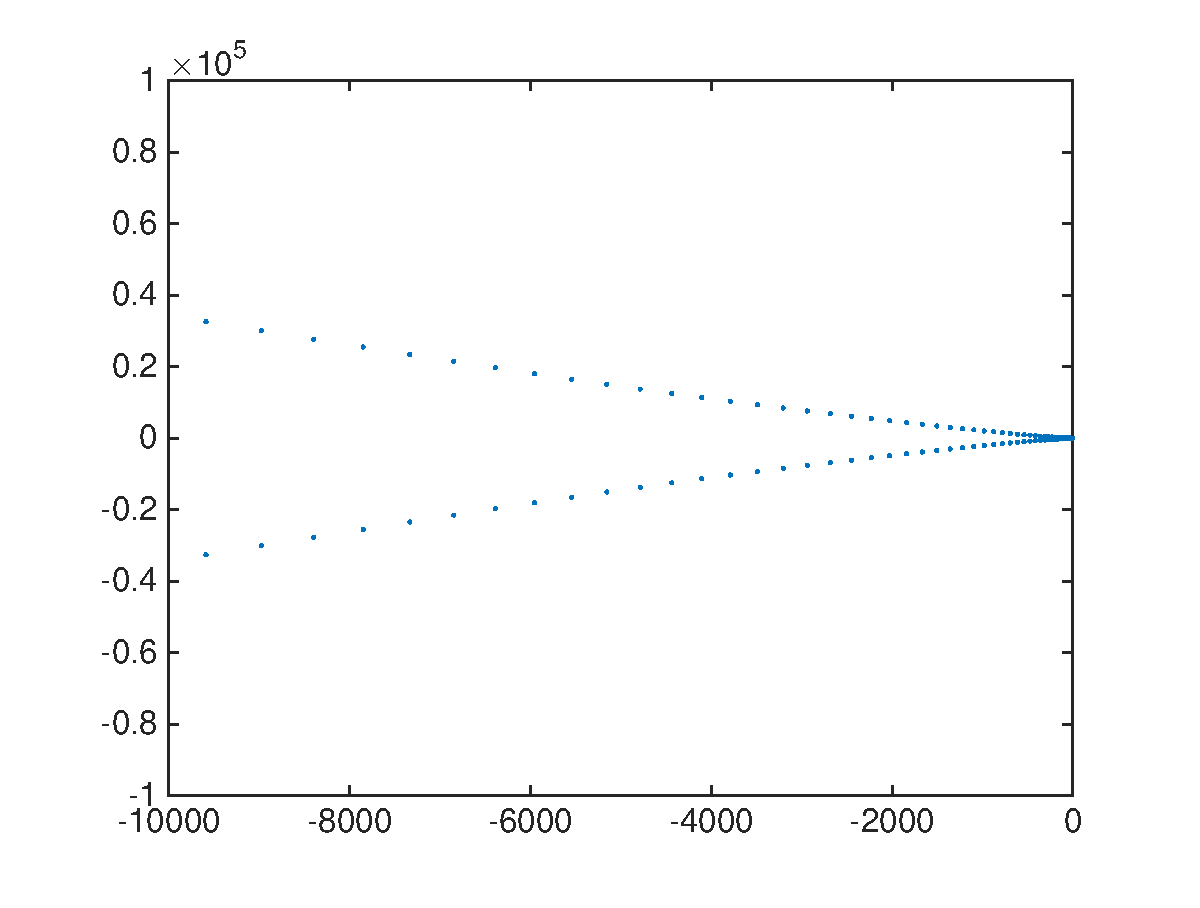
\includegraphics[width=8.5cm]{cheb10ud2_2}
	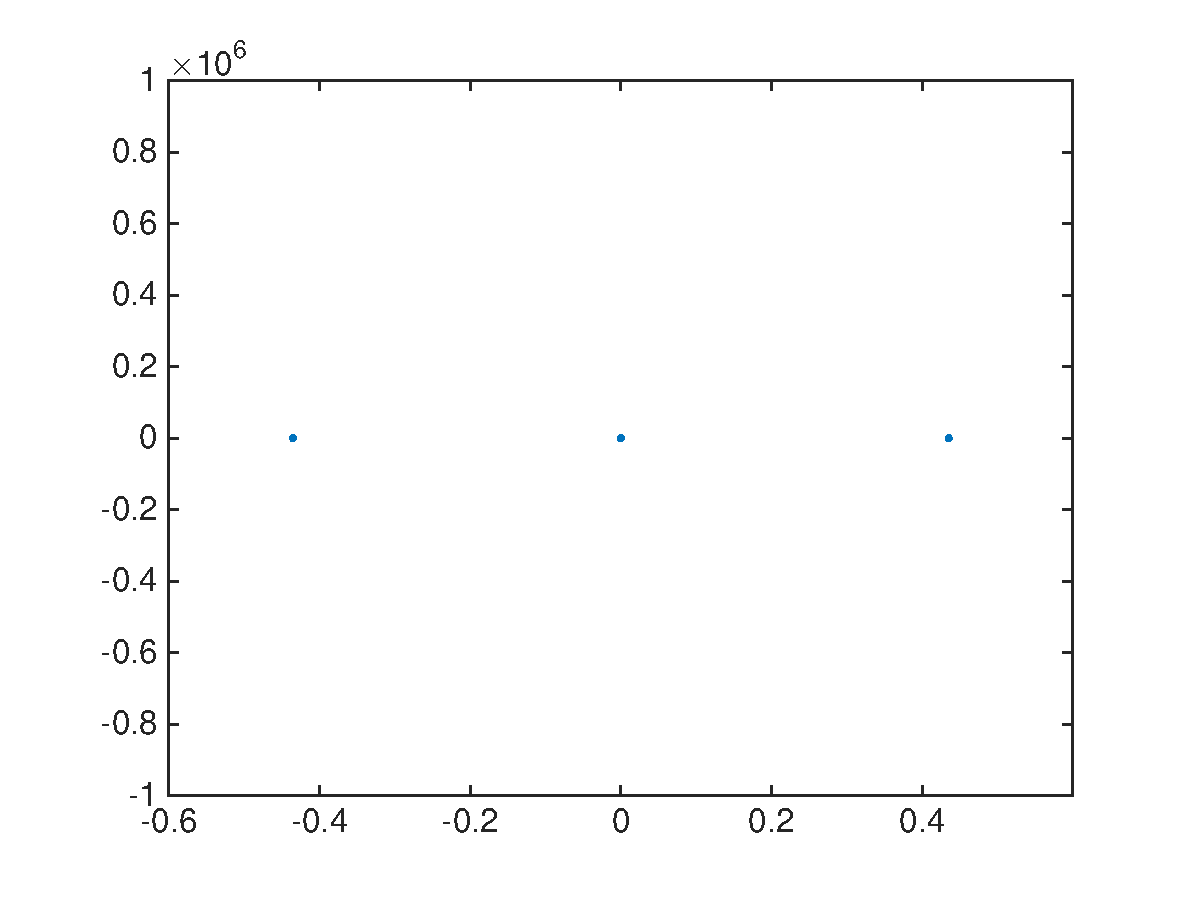
\includegraphics[width=8.5cm]{cheb10ud2_2zoom}
	\caption{Spectrum of linearization \eqref{linear5th} of 5th order PDE \eqref{KdV5travel} about double pulse 2(2). Plot on left shows the absolute spectrum. Plot on right is zoom around origin, showing eigenvalues near 0. Wave speed $c = 10$, Chebyshev spectral methods, $N = 257$.}
\end{figure}

The eigenvalues near 0 for the first four double pulses are given below. They are very similar to those in the Fourier case.

\begin{table}[H]
\begin{tabular}{l|lll}
 Double Pulse   & $c = 10$            & $c=7.5$                        & $c=5$        \\ \hline
  2(2) &     $\pm 0.4352$             & $\pm 0.2730$                   & $\pm 0.1363$ \\ 
  2(3) &     3.5702e-08 $\pm 0.0691i$ & 1.2186e-08 $\pm 0.0413i$       & 2.0229e-09 $\pm 0.0190i$\\ 
  2(4) &     $\pm 0.0109$             & $\pm 0.0064$                   & \\ 
  2(5) &    -2.4222e-12 $\pm 0.0020i$ & 8.0169e-13 $\pm$ 9.4458e-04$i$ & \\
\end{tabular}
\caption{Eigenvalues for linearization \eqref{linear5th} of 5th order PDE \eqref{KdV5travel} about double pulses 2(2), 2(3), 2(4), and 2(5) for wave speeds $c = 10, 7.5, 5$. Chebyshev spectral methods, $N = 257$.}
\end{table}

As with Fourier spectral methods, we can use \texttt{fsolve} to eliminate the small real part of the eigenvalues for double pulses 2(3) and 2(5). In this case, we get an even larger improvement in $\max{|Jv - \lambda v|}$ when we do this.

\begin{table}[H]
\begin{tabular}{l|ll}
 Double Pulse   & $\max{|Lv - \lambda v|}$ before \texttt{fsolve} & $\max{|Lv - \lambda v|}$ after \texttt{fsolve}\\ \hline
  2(3) & 3.0291e-06 & 8.5938e-09 \\
  2(5) & 1.1501e-06 & 1.2419e-10 \\
\end{tabular}
\caption{Maximum of eigenvalue problem $|Lv - \lambda v|$ before and after using Matlab's \texttt{fsolve} to eliminate small real part of eigenvalue. Wave speed $c = 10$, Chebyshev spectral methods, $N = 257$.}
\end{table}

\subsection{Time stepping}

In this section, we perform timestepping using the 5th order KdV equation \eqref{KdV5travel}. We write this equation as 
\begin{equation} \label{KdV5separated}
u_t = Lu + F(u)
\end{equation}
where $L = \partial_x^5 - \partial_x^3 + c \partial_x$ is the linear part of \eqref{KdV5travel}, and $F(u) = -2 u u_x$ is the nonlinear part.\\

A standard scheme in the literature is a 4th-order Runge-Kutta scheme using an integrating factor. However, this scheme requires a very small time step to be stable, and this is not practical for longer time integrations. For this reason, we use here a  Crank-Nicoloson/Adams-Bashforth 2 IMEX scheme.

\begin{equation}\label{scheme}
\frac{u^{n+1} - u^n}{k} = \frac{3}{2}F(u^n) - \frac{1}{2}F(u^{n-1}) + \frac{1}{2}\left(Lu^{n+1} - Lu^n \right) 
\end{equation}

where $u^n$ represents the $n$th time step, and $k$ is the time step size. We choose $k = 0.01$ for our time step. For spatial discretization, we use Chebyshev spectral methods, since with Fourier spectral methods we incorporate additional high-frequency oscillations into our solution as a consequence of the essential spectrum on the imaginary axis. We use wave speed $c = 10$ and $N = 257$ Chebyshev-Gauss-Lobatto nodes. Since we now have a 5th order equation, we need a 5th boundary condition. Since for $\textrm{Re} \lambda > 0$ there are three spatial eigenvalues with positive real part and only two with negative real part, we choose a homogeneous Neumann boundary condition for the 2nd derivative on the right boundary (TO BE HONEST, I STILL DON'T REALLY UNDERSTAND THIS IN A MEANINGFUL WAY). In this case, we take our interpolating polynomial to be of the form $p(x) = (L-x)^2 (L+x) q(x)$, where $q(x)$ is degree $\leq N-3$ and $q(\pm L) = 0$. \\

First we perform timestepping starting at our equilibrium solution of double pulse 2(3). If we plot the distance between the pulses vs time, we see some very small amplitude oscillations with frequency 0.0691, which is imaginary part of the eigenvalue of the linearization. This is shown in the figure below.

\begin{figure}[H]
	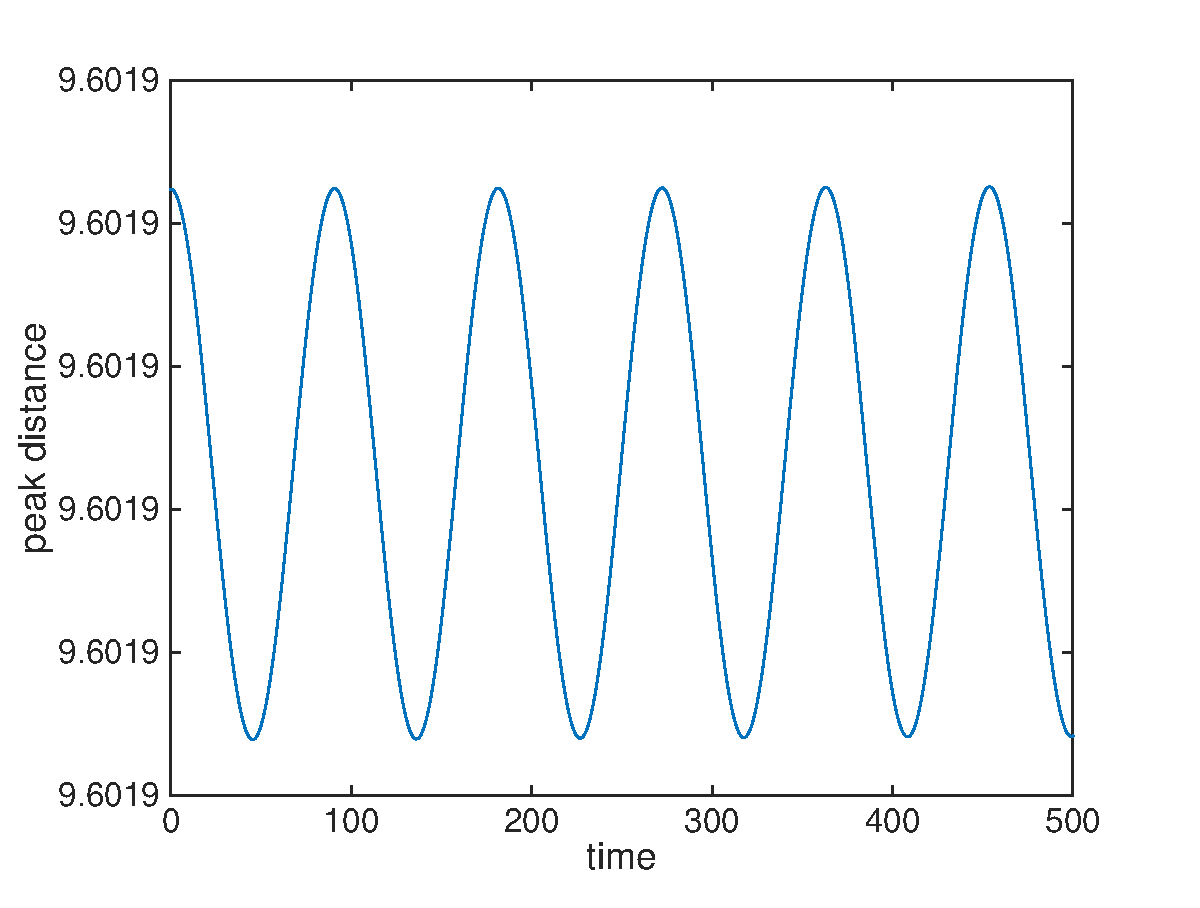
\includegraphics[width=8.5cm]{cheb10dist2_0}
	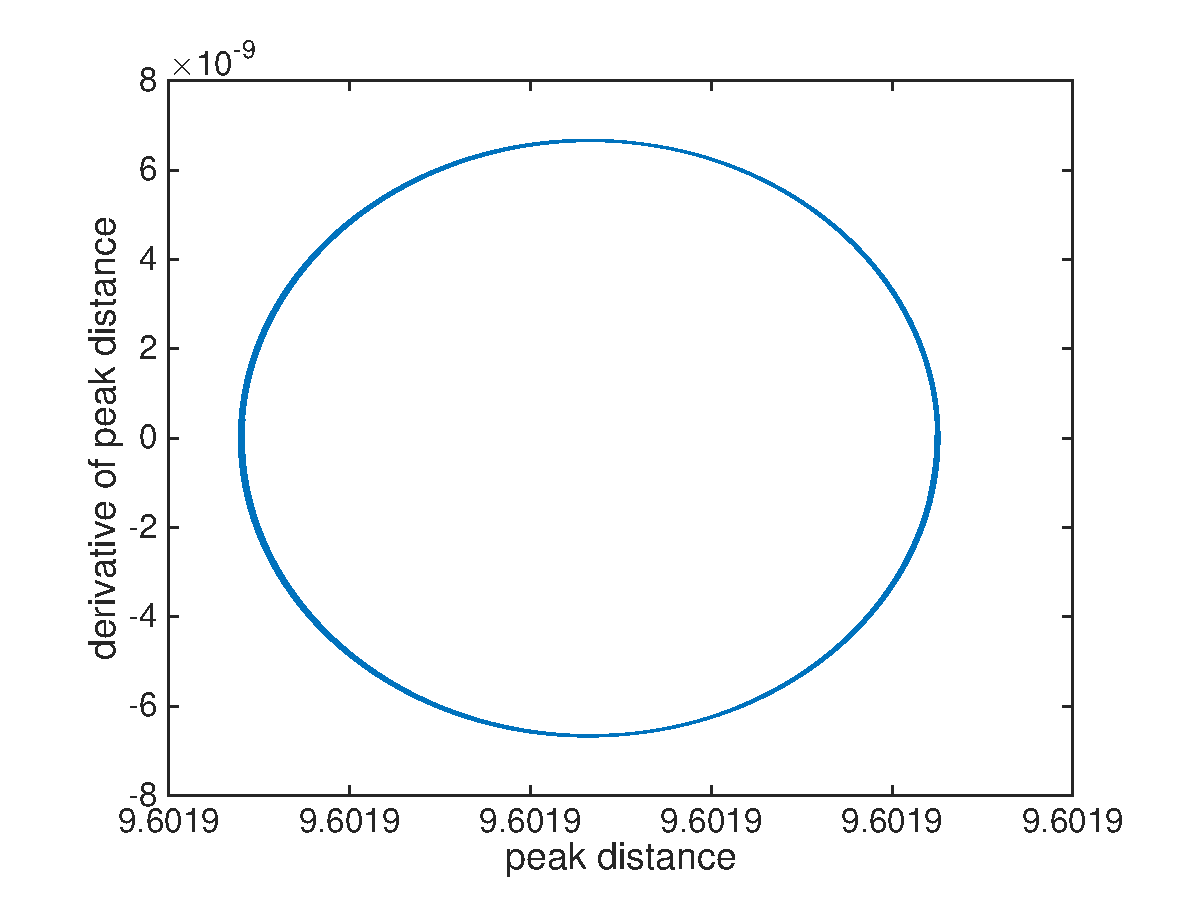
\includegraphics[width=8.5cm]{cheb10deriv2_0}
	\caption{Timestepping with initial condition pulse 2(3). Plot of distance between pulses vs time (left) and derivative of distance vs distance between pulses (right). Period of oscillations is 90.8750, frequency of oscillations is 0.0691, which is the imaginary part of the eigenvalue of the linearization about pulse 2(3). Wave speed $c = 10$, Chebyshev spectral methods, $N = 257$.}
\end{figure}

Next we perform timestepping starting at perturbations of our double pulse solutions. Since it appears that the pulse distance is a parameter of interest (NO IDEA WHY WE THOUGHT THIS WAS THE CASE, BUT SEEMS TO BE TRUE, SOMETHING ABOUT A CENTER MANIFOLD REDUCTION BEING POSSIBLE IF THE EIGENVALUES ARE PURE IMAGINARY), we will perturb our double pulse solutions by pulling the double pulses apart. We accomplish this by adding a small constant segment between the two pulses. Doing this introduces some translation into the system, but we can eliminate this by changing the wave speed $c$. We do this for many different double pulses and amounts of stretching and obtain the following phase portrait. We have reduced the system to two dimensions: the distance between the two pulses ($x$-axis) and the derivative of this distance ($y$-axis).

\begin{figure}[H]
	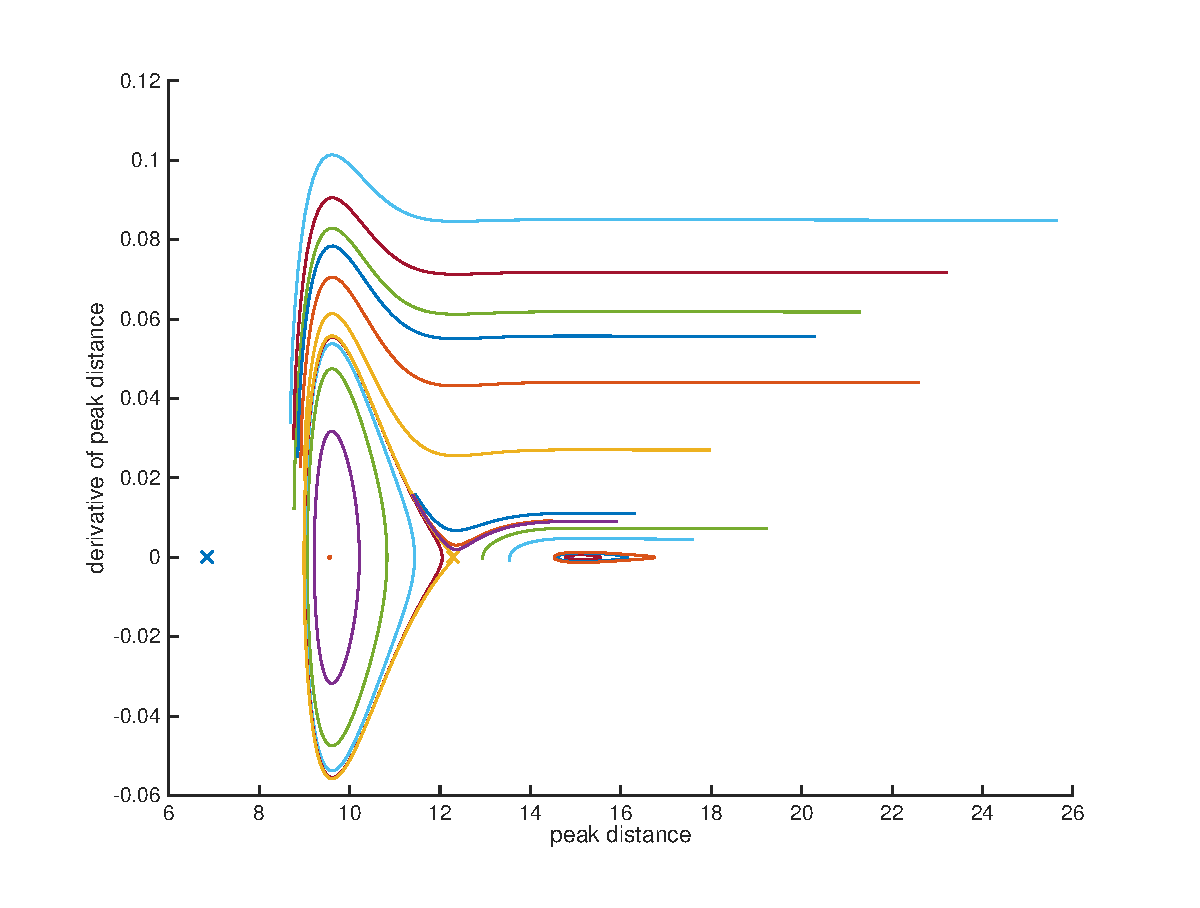
\includegraphics[width=8.5cm]{phaseportrait1}
	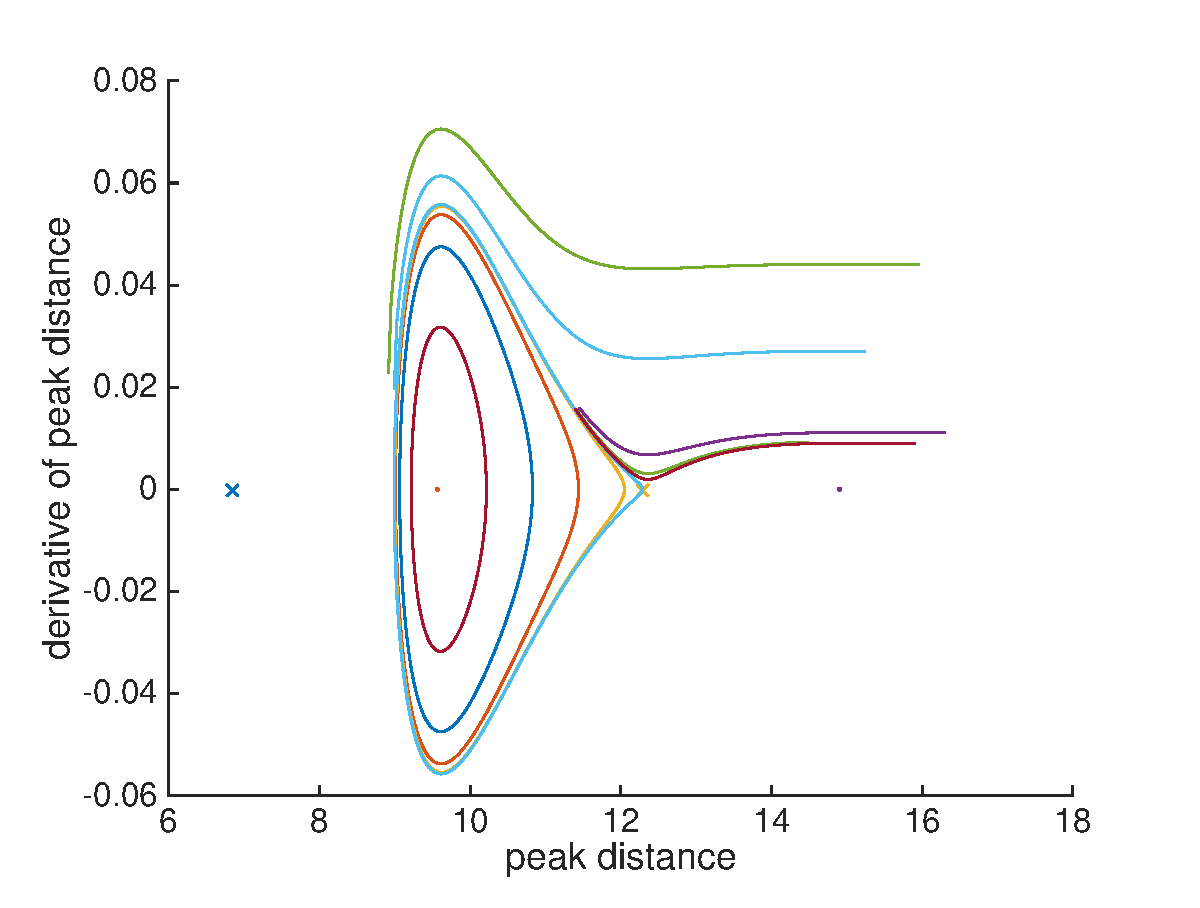
\includegraphics[width=8.5cm]{phaseportrait2}
	\caption{Phase portrait for reduced two-dimensional system. Variables are distance between two pulses and its derivative. Wave speed $c = 10$, Chebyshev spectral methods, $N = 256$. Time step size 0.01.}
\end{figure}

This looks very similar to the phase portrait of the simplified, two-dimensional system \eqref{simplesystem}. In the simple phase portrait, (0,0) is the equilibrium corresponding to pulse 2(2). 

\begin{figure}[H]
	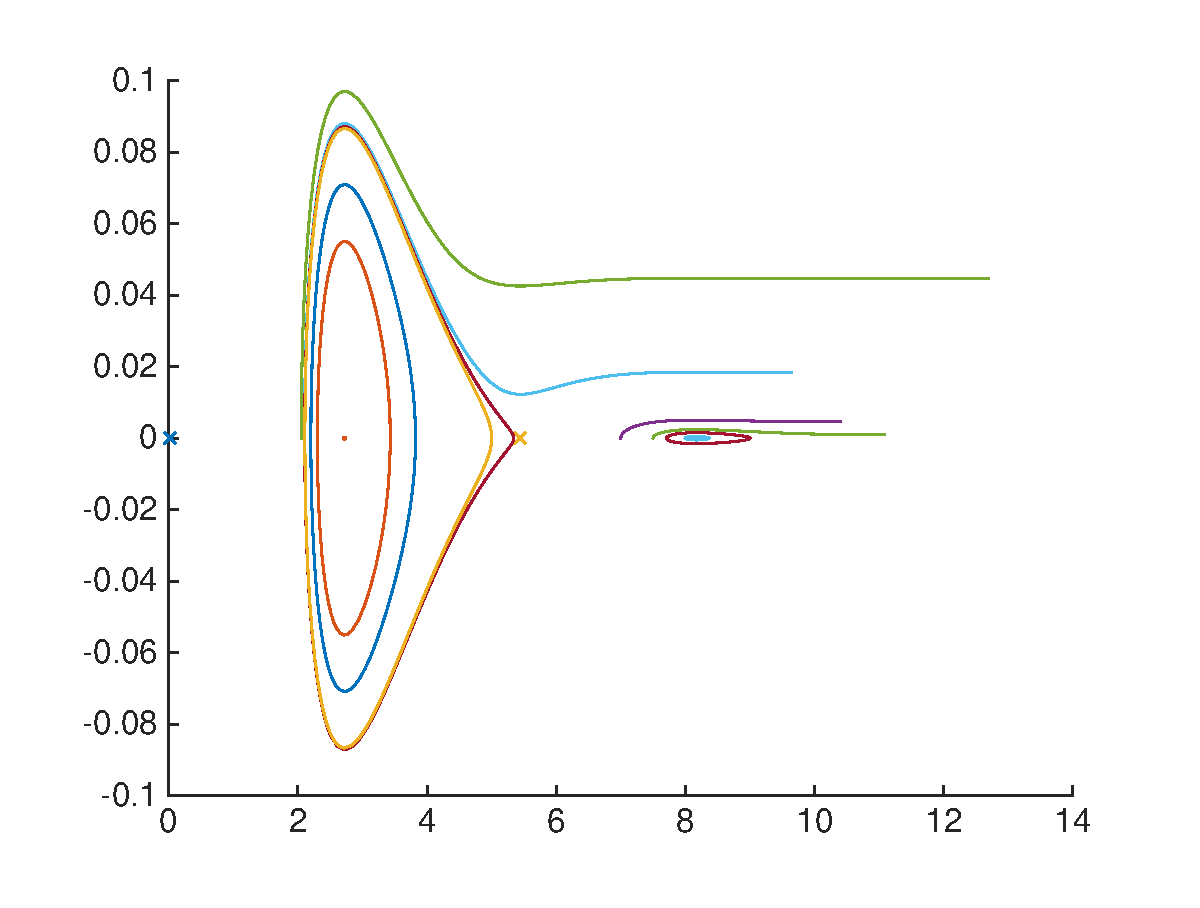
\includegraphics[width=8.5cm]{simplephaseportrait}
	\caption{Phase portrait for simplified system. Integration performed using Matlab's \texttt{ode45}.}
\end{figure}

\subsection{Multipulses}

We conclude with a brief look at multipulses. We can construct these using similar techniques to those we used above. We actually start with the double pulses when constructing these since they are closer to the multipulses we seek. Here are 3- and 4-pulses based on pulse 2(2) using Fourier spectral methods.

\begin{figure}[H]
	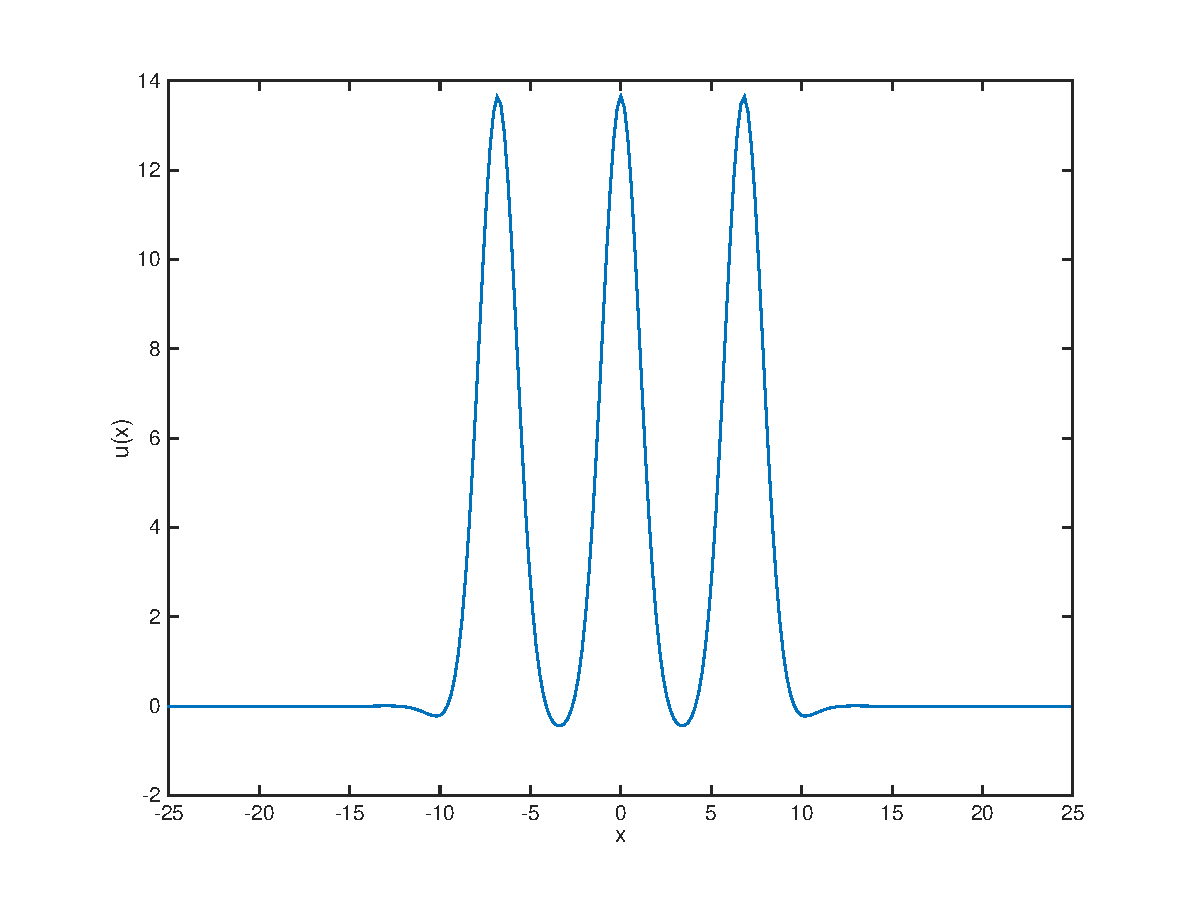
\includegraphics[width=8.5cm]{four10um1_3}
	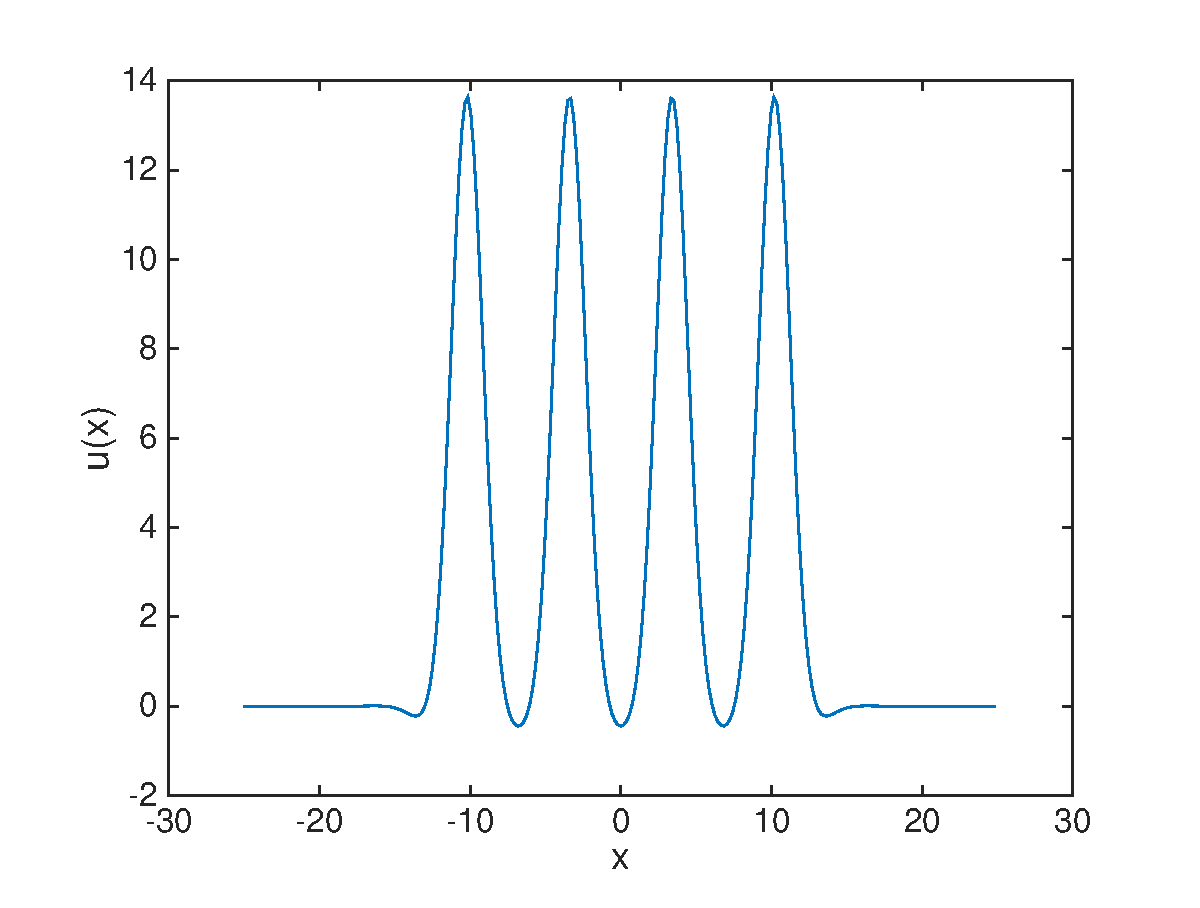
\includegraphics[width=8.5cm]{four10um1_4.eps}
	\caption{Multipulses 3(2,2) and 4(2,2,2). Wave speed $c = 10$, Fourier spectral methods, $N = 256$.}
\end{figure}

Below we see their eigenvalues. We have two additional eigenvalues (which are negatives of each other) for each additional pulse.

\begin{figure}[H]
	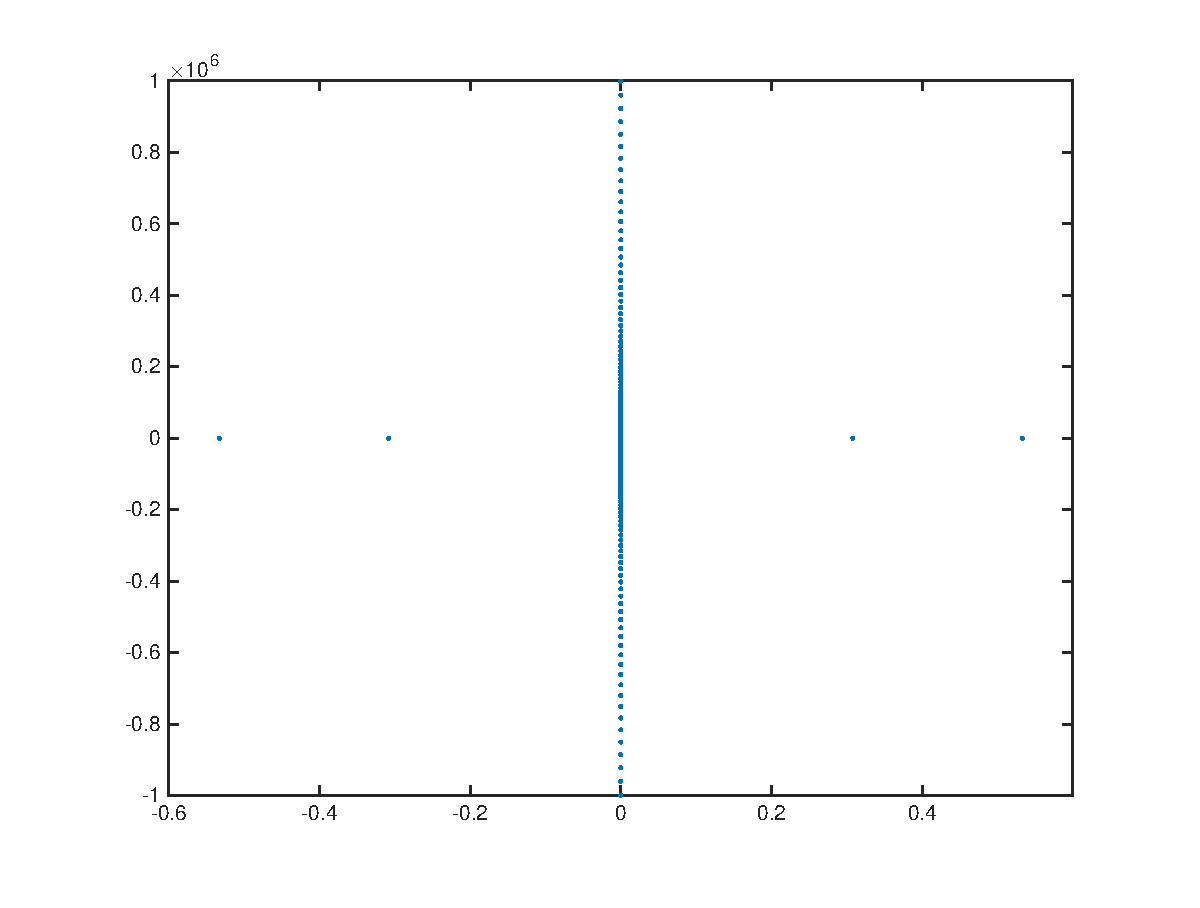
\includegraphics[width=8.5cm]{four10um1_3lambda}
	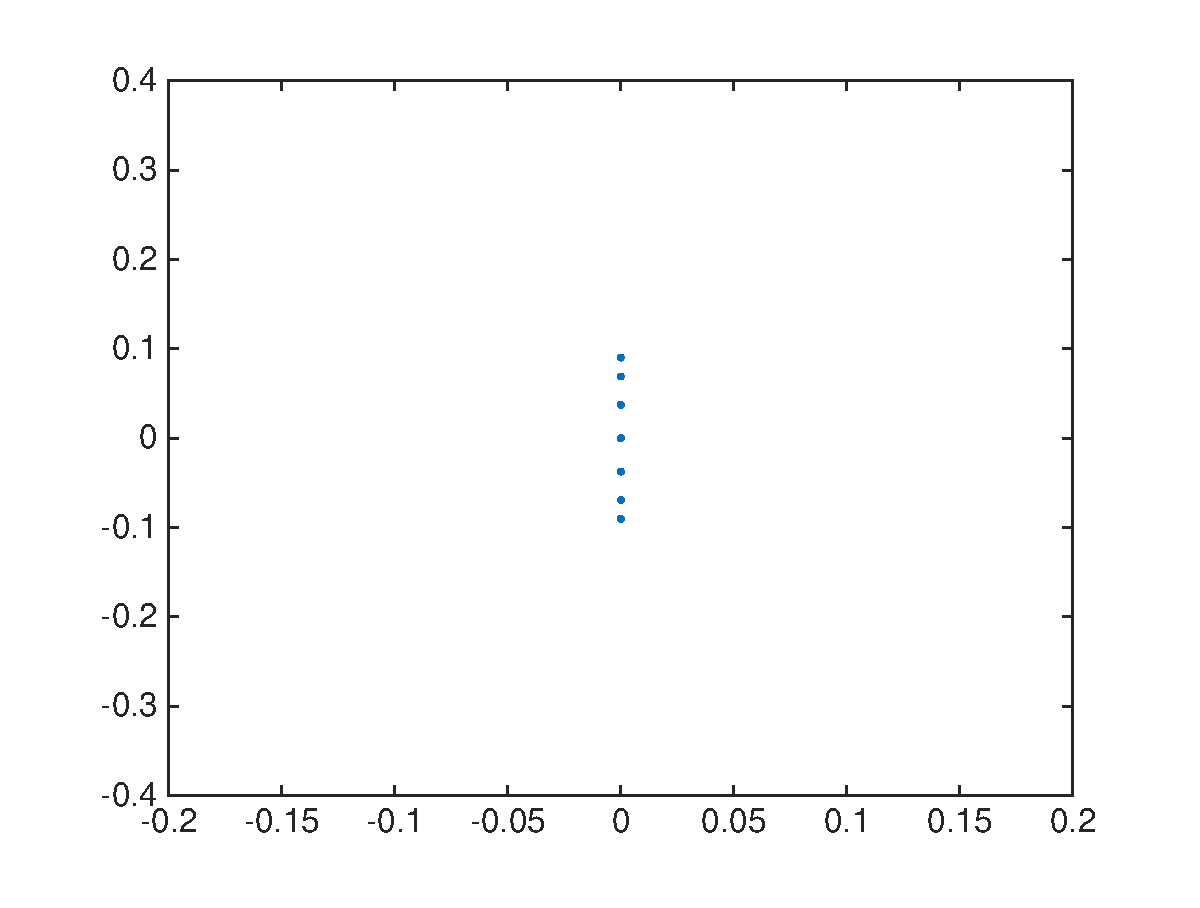
\includegraphics[width=8.5cm]{four10um1_4lambda}
	\caption{Eigenvalues of 5th order KdV for multipulses 3(2,2) and 4(2,2,2). Wave speed $c = 10$, Fourier spectral methods, $N = 256$.}
\end{figure}

\begin{table}[H]
\begin{tabular}{l|l}
  Pulse    &  Nonzero Eigenvalues \\ \hline
  2(2)     &     $\pm 0.4352$  \\ 
  3(2,2)   &     $\pm 0.5328, \pm 0.3079$   \\ 
  4(2,2,2) &     $\pm 0.5683, \pm 0.4353, \pm 0.2358 $  \\ 
\end{tabular}
\caption{Eigenvalues of 5th order KdV for multipulses 3(2,2) and 4(2,2,2). Wave speed $c = 10$, Fourier spectral methods, $N = 256$.}
\end{table}

 Here are 3- and 4-pulses based on pulse 2(3), this time using Chebyshev spectral methods.

\begin{figure}[H]
	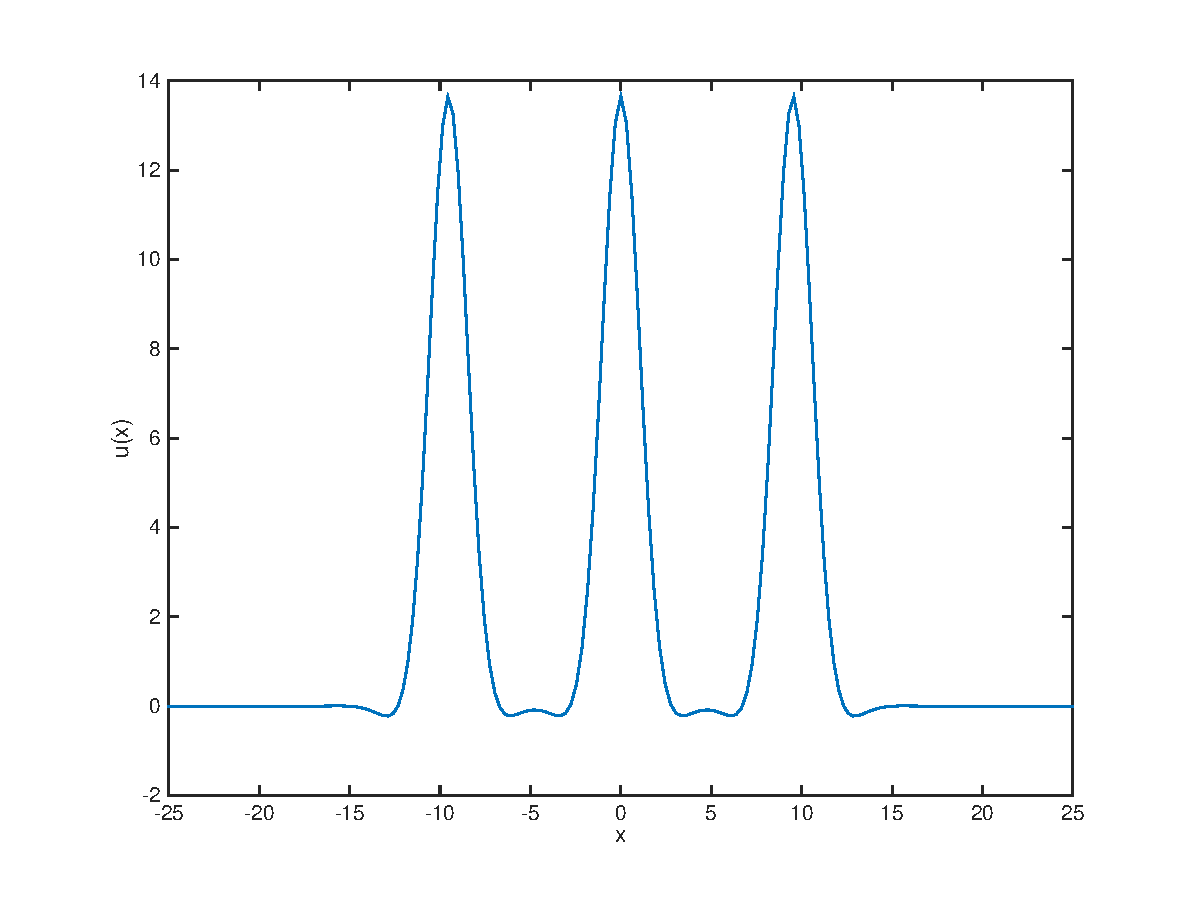
\includegraphics[width=8.5cm]{cheb10um2_3.eps}
	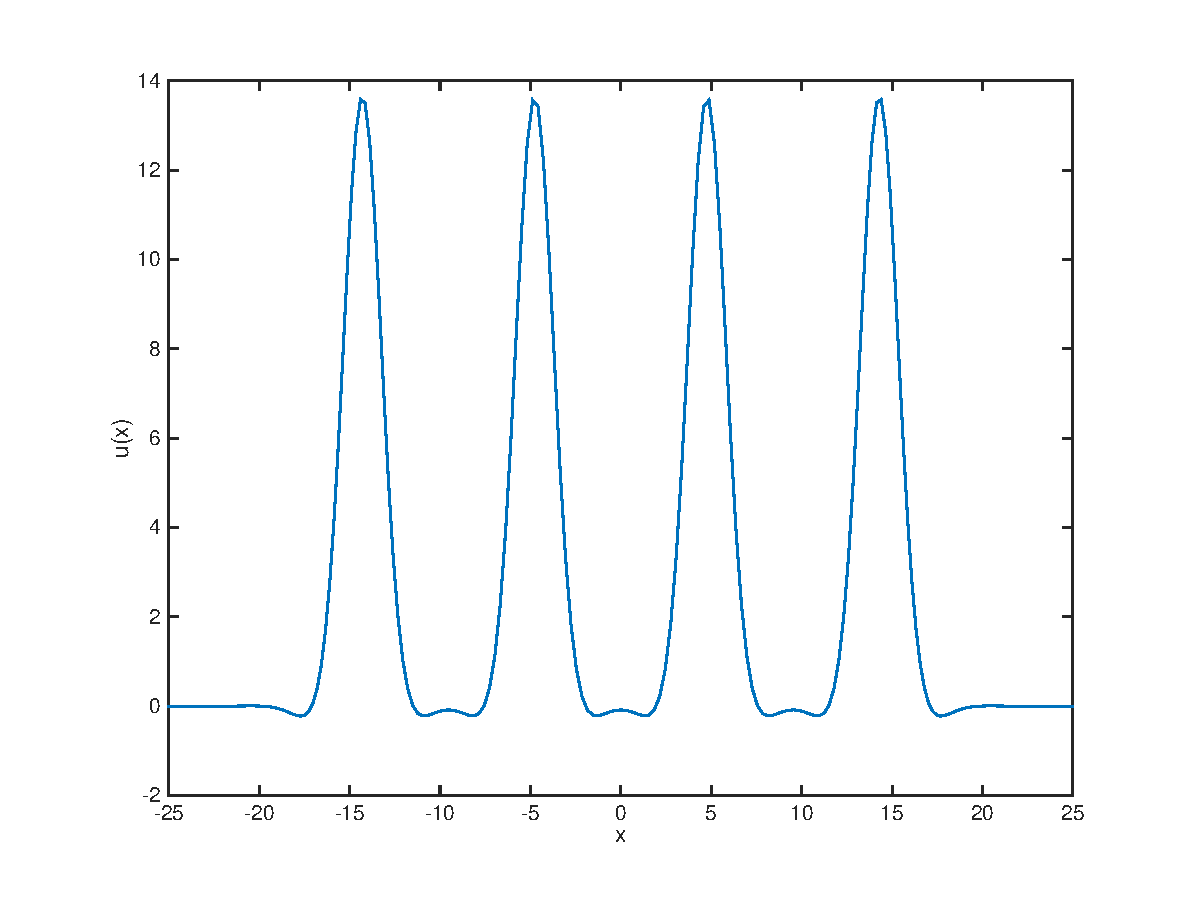
\includegraphics[width=8.5cm]{cheb10um2_4.eps}
	\caption{Multipulses 3(3,3) and 4(3,3,3). Wave speed $c = 10$, Chebyshev spectral methods, $N = 257$.}
\end{figure}

Here are the eigenvalues near the origin for these multipulses. Note that there is an additional complex-conjugate pair of eigenvalues for each additional pulse.

\begin{figure}[H]
	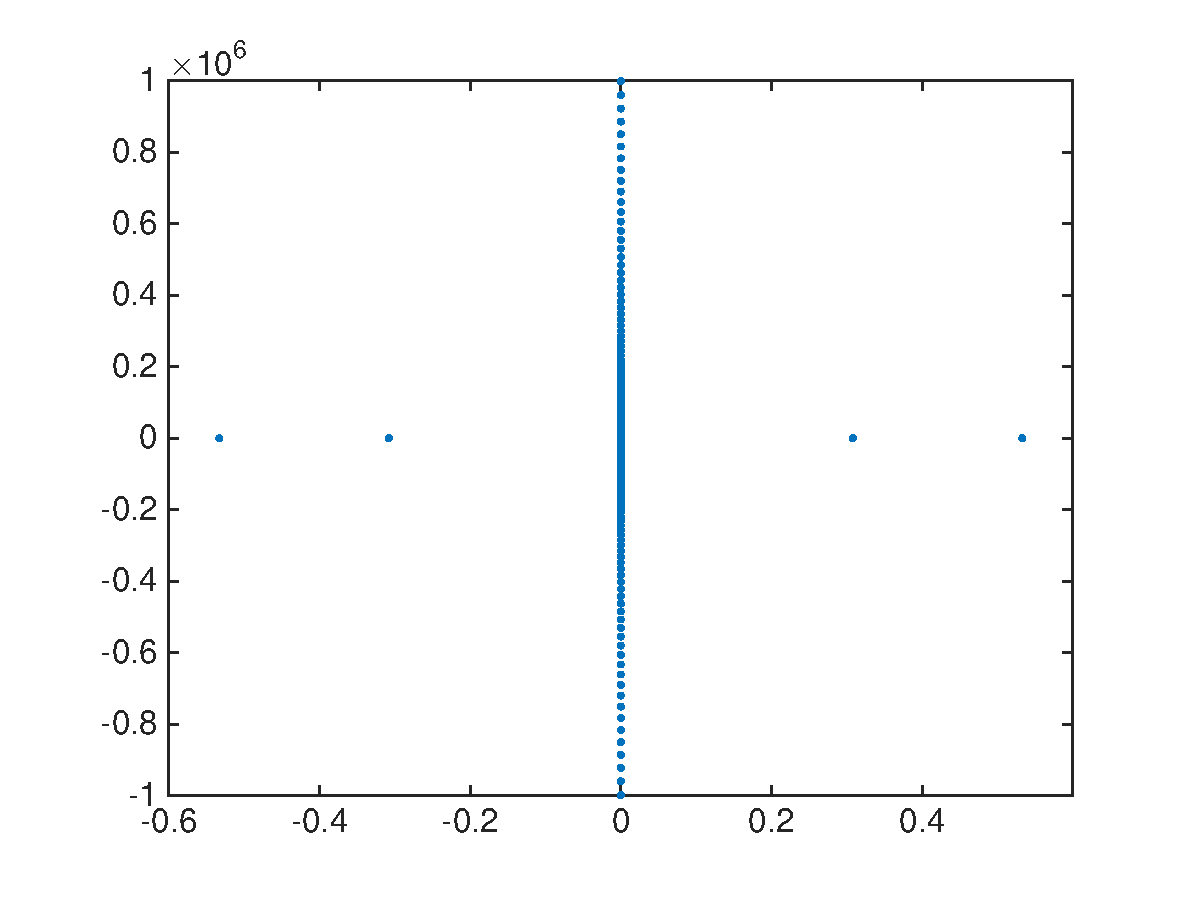
\includegraphics[width=8.5cm]{cheb10um2_3lambda.eps}
	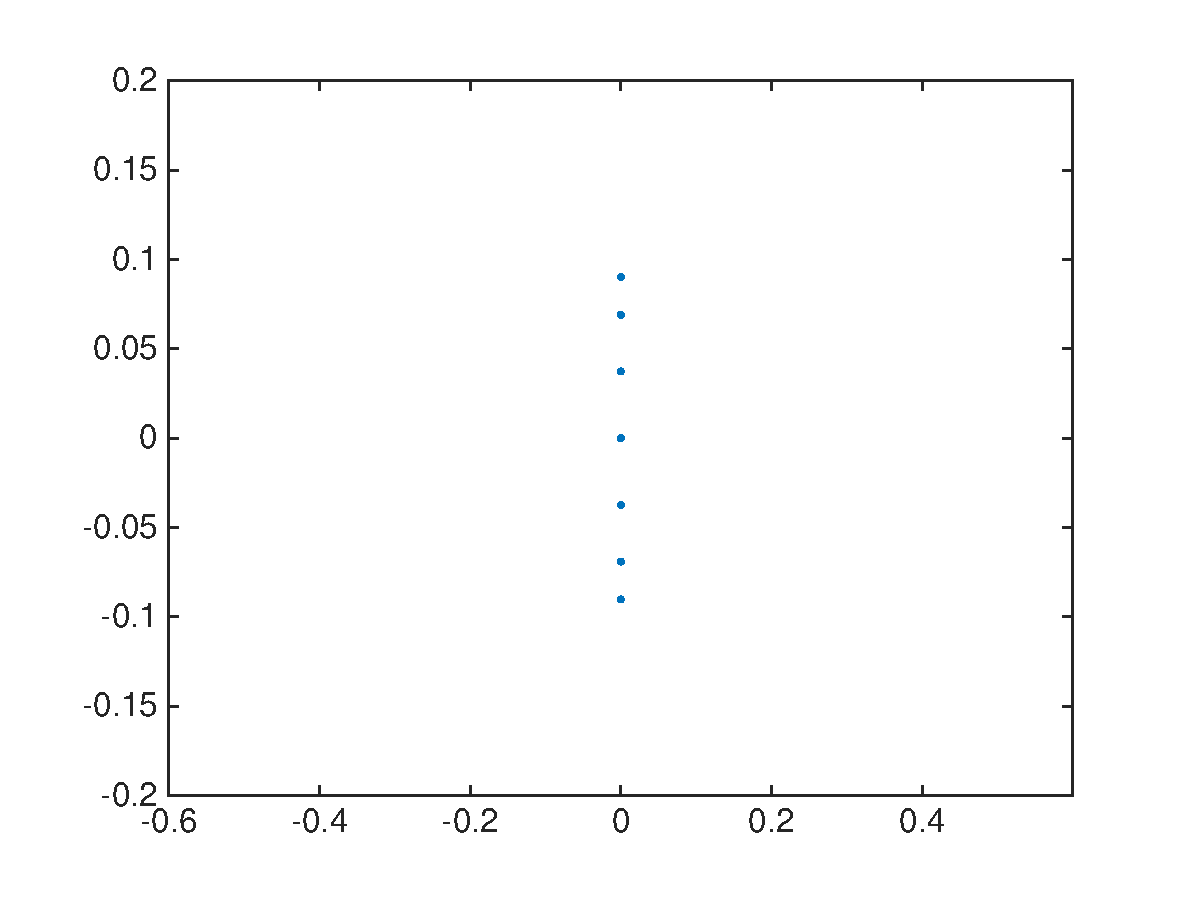
\includegraphics[width=8.5cm]{cheb10um2_4lambda.eps}
	\caption{Eigenvalues near origin of 5th order KdV for multipulses 3(3,3) and 4(3,3,3). Wave speed $c = 10$, Chebyshev spectral methods, $N = 257$.}
\end{figure}

Here are the imaginary parts of the eigenvalues for linearization about these multipulses. In all cases, Matlab's \texttt{eig} yields a small real part which can be eliminated using \texttt{fsolve} by following the same procedure as with the double pulses.

\begin{table}[H]
\begin{tabular}{l|l}
  Pulse    &  Nonzero Eigenvalues \\ \hline
  2(3)     &     $\pm 0.0691i$ \\ 
  3(3,3)   &     $\pm 0.0846i$, $\pm 0.0489i$   \\ 
  4(3,3,3) &     $\pm 0.0903i$, $\pm 0.0691i$, $\pm 0.0374i$ \\ 
\end{tabular}
\caption{Eigenvalues of 5th order KdV for multipulses 3(3,3) and 4(3,3,3). Tiny real part of eigenvalues found by \texttt{eig} has been removed using \texttt{fsolve}, with improvement in $\max{|Jv - \lambda v|}$. Wave speed $c = 10$, Chebyshev spectral methods, $N = 257$.}
\end{table}

\printbibliography

\end{document}